% =====================================================================
% Online Auction System — Diploma Thesis
% MUST Format — Compile with: xelatex thesis.tex
% =====================================================================
\documentclass[12pt, a4paper]{report}

% ── Unicode / Font ────────────────────────────────────────────────────
\usepackage{fontspec}
\setmainfont{Times New Roman}
\setsansfont{Arial}
\setmonofont{Courier New}

% ── Page layout ───────────────────────────────────────────────────────
\usepackage[
  top=25mm, bottom=25mm,
  left=30mm, right=20mm
]{geometry}

% ── Language ──────────────────────────────────────────────────────────
\usepackage{polyglossia}
\setdefaultlanguage{english}
\setotherlanguage{russian}

% ── Typography ────────────────────────────────────────────────────────
\usepackage{setspace}
\onehalfspacing
\usepackage{parskip}
\setlength{\parindent}{1.25cm}
\setlength{\parskip}{0pt}

% ── Color & page color ────────────────────────────────────────────────
\usepackage[table]{xcolor}
\definecolor{Cover}{RGB}{102,255,255}    % MUST cyan-blue cover
\definecolor{OliveGreen}{cmyk}{0.64,0,0.95,0.40}
\definecolor{CadetBlue}{cmyk}{0.62,0.57,0.23,0}
\definecolor{lightlightgray}{gray}{0.9}
\definecolor{codebg}{rgb}{0.97,0.97,0.97}
\definecolor{codeframe}{rgb}{0.85,0.85,0.85}
\definecolor{codecomment}{rgb}{0.40,0.40,0.40}
\definecolor{codestring}{rgb}{0.16,0.51,0.20}
\definecolor{codekeyword}{rgb}{0.08,0.22,0.72}

% ── Tables ────────────────────────────────────────────────────────────
\usepackage{booktabs}
\usepackage{longtable}
\usepackage{array}
\usepackage{tabularx}
\newcolumntype{L}[1]{>{\raggedright\arraybackslash}p{#1}}
\newcolumntype{C}[1]{>{\centering\arraybackslash}p{#1}}

% ── Figures ───────────────────────────────────────────────────────────
\usepackage{graphicx}
\graphicspath{{./}}
\usepackage{float}
\usepackage{caption}
\captionsetup{font=small, labelfont=bf}
\usepackage{tikz}

% ── Code listings ─────────────────────────────────────────────────────
\usepackage{listings}

% JavaScript is not built-in to listings — define it here
\lstdefinelanguage{JavaScript}{
  keywords={break,case,catch,continue,debugger,default,delete,do,else,
             false,finally,for,function,if,in,instanceof,new,null,return,
             switch,this,throw,true,try,typeof,var,void,while,with,
             let,const,async,await,of,class,extends,import,export,from},
  morecomment=[l]{//},
  morecomment=[s]{/*}{*/},
  morestring=[b]',
  morestring=[b]"
}

\lstset{
  backgroundcolor=\color{codebg},
  frame=single,
  rulecolor=\color{codeframe},
  basicstyle=\small\ttfamily,
  keywordstyle=\color{codekeyword}\bfseries,
  commentstyle=\color{codecomment}\itshape,
  stringstyle=\color{codestring},
  numbers=left,
  numberstyle=\tiny\color{gray},
  numbersep=8pt,
  breaklines=true,
  breakatwhitespace=true,
  tabsize=2,
  showstringspaces=false,
  language=JavaScript
}

% ── Hyperlinks ────────────────────────────────────────────────────────
\usepackage[
  colorlinks=true,
  linkcolor=black,
  urlcolor=blue,
  citecolor=black
]{hyperref}

% ── Misc ──────────────────────────────────────────────────────────────
\usepackage{amsmath}
\usepackage{enumitem}
\usepackage{titlesec}
\usepackage{fancyhdr}
\usepackage{tocloft}
\usepackage{pifont}
\usepackage{afterpage}

% ── Chapter / section titles ──────────────────────────────────────────
\titleformat{\chapter}[block]
  {\normalfont\Large\bfseries}{\thechapter.}{1em}{}
\titlespacing*{\chapter}{0pt}{20pt}{10pt}

\titleformat{\section}
  {\normalfont\large\bfseries}{\thesection}{1em}{}
\titleformat{\subsection}
  {\normalfont\normalsize\bfseries}{\thesubsection}{1em}{}

% ── Headers / footers ─────────────────────────────────────────────────
\setlength{\headheight}{14pt}
\pagestyle{fancy}
\fancyhf{}
\fancyhead[R]{\small\leftmark}
\fancyfoot[C]{\thepage}
\renewcommand{\headrulewidth}{0.4pt}

% ── Helper ────────────────────────────────────────────────────────────
\newcommand{\imgplaceholder}[2]{%
  \begin{center}
    \fbox{\parbox{0.7\linewidth}{\centering\vspace{12pt}
      [Зураг: \textit{#1}]\\[4pt]
      \small #2\vspace{12pt}}}
  \end{center}
}

% ── Thesis metadata ───────────────────────────────────────────────────
\newcommand{\thesistitle}{Дуудлага худалдааны систем /мобайл вэб хамт/}
\newcommand{\thesistype}{Бакалаврын төгсөлтийн ажил}
\newcommand{\authorlong}{Түвшинзаяа Бөхбилэгт}
\newcommand{\authorshort}{Т.Бөхбилэгт}
\newcommand{\supervisor}{Доктор (Ph.D), П.Энхтайван}
\newcommand{\deptchair}{Доктор (Ph.D), Дэд профессор, А.Алтангэрэл}
\newcommand{\universityname}{Шинжлэх Ухаан Технологийн Их Сургууль}
\newcommand{\facultyname}{Мэдээлэл, Холбооны Технологийн Сургууль}
\newcommand{\deptname}{Мэдээллийн технологийн тэнхим}
\newcommand{\degreeid}{D061304}
\newcommand{\degreename}{Мэдээллийн технологи}
\newcommand{\authormail}{buhuu1125@gmail.com}

% =====================================================================
\begin{document}

% ── Front matter numbering ────────────────────────────────────────────
\pagenumbering{roman}
\pagestyle{plain}

% =====================================================================
%  PAGE 1 — BLUE COVER (MUST FORMAT)
% =====================================================================
\begin{titlepage}
% Full-page cyan background (tikz — reliable across all engines)
\begin{tikzpicture}[remember picture, overlay]
  \fill[Cover] (current page.south west) rectangle (current page.north east);
\end{tikzpicture}
\begin{center}

{\scshape\LARGE \universityname}\\[0.3cm]
{\scshape\Large \facultyname}\\[0.5cm]

% Logo — no float wrapper inside titlepage

\includegraphics[scale=0.2]{MUST_logo}\\[0.8cm]

\hfill{\large \authorlong}

\vspace{0.8cm}
{\huge\bfseries \thesistitle}

\vspace{3cm}
{\Large\textsc{\thesistype}}

\vfill
{\large Улаанбаатар хот}

\end{center}
\end{titlepage}

% =====================================================================
%  PAGE 2 — SUBTITLE / INFO PAGE
% =====================================================================
\begin{titlepage}
\begin{center}

{\scshape\LARGE \universityname}\\[0.3cm]
{\scshape\Large \facultyname}\\[0.5cm]

\vspace{1.5cm}
\hfill{\large \deptname}

\vspace{1.5cm}
{\huge\bfseries \thesistitle}

\vspace{1.5cm}

\begin{minipage}[t]{0.9\textwidth}
\begin{flushleft}
\normalsize
Мэргэжлийн индекс: \degreeid \\
Мэргэжил: \degreename \\[2cm]

\emph{Удирдагч:} \supervisor \\
\emph{Гүйцэтгэгч:} \authorshort \\
\end{flushleft}
\end{minipage}

\vfill
{\large Улаанбаатар хот} \\
{\large 2026 он 1 сар}

\end{center}
\end{titlepage}

% =====================================================================
%  PAGE 3–4 — WORK PLAN, PROGRESS & REVIEW FORM
% =====================================================================
\begin{titlepage}

\vspace*{0.5cm}
Батлав. \deptname-ийн эрхлэгч:
\begin{flushright}
\makebox[4cm]{\dotfill} /\deptchair/
\end{flushright}

Удирдагч:
\begin{flushright}
\makebox[4cm]{\dotfill} /\supervisor/
\end{flushright}

\begin{center}

\vspace*{1.5cm}
\textbf{{\large ТӨГСӨЛТИЙН АЖЛЫН ТӨЛӨВЛӨГӨӨ}}\\[0.5cm]

\textsc{\large Сэдэв: ``\thesistitle''}\\[0.5cm]

\begin{tabular}{|c|p{7cm}|c|c|}
\hline
№ & \makebox[7cm][c]{Ажлын бүлэг, хэсгийн нэр} & Эзлэх хувь & Дуусах хугацаа \\ \hline
1 & Удиртгал         &  5\% & 2025-03-05 \\ \hline
2 & Онолын хэсэг     & 20\% & 2025-03-30 \\ \hline
3 & Судалгааны хэсэг & 30\% & 2025-04-15 \\ \hline
4 & Төслийн хэсэг    & 35\% & 2025-05-20 \\ \hline
5 & Дүгнэлт          & 10\% & 2025-05-24 \\ \hline
\end{tabular}

\vspace{1.5cm}
Төлөвлөгөөг боловсруулсан оюутан: \makebox[3cm]{\dotfill} /\authorshort/

\end{center}

\newpage

\begin{center}

\vspace*{1.5cm}
\textbf{{\large ТӨГСӨЛТИЙН АЖЛЫН ЯВЦ}}\\[0.5cm]

\begin{tabular}{|c|p{7cm}|c|c|}
\hline
№ & \makebox[7cm][c]{Хийж гүйцэтгэсэн ажил} & Биелсэн хугацаа & Удирдагчийн гарын үсэг \\ \hline
1 & Удиртгал         & 2025-03-05 & \\ \hline
2 & Онолын хэсэг     & 2025-03-30 & \\ \hline
3 & Судалгааны хэсэг & 2025-04-15 & \\ \hline
4 & Төслийн хэсэг    & 2025-05-20 & \\ \hline
5 & Дүгнэлт          & 2025-05-24 & \\ \hline
\end{tabular}

\vspace{0.8cm}
Ажлын товч дүгнэлт \\[0.4cm]
\dotfill \\[0.2cm]
\dotfill \\[0.2cm]
\dotfill \\[0.2cm]
\dotfill \\[0.2cm]
\dotfill \\[0.2cm]
\dotfill \\[0.4cm]
Удирдагч: \makebox[3cm]{\dotfill} /\supervisor/ \\

\vspace{1.5cm}
ЗӨВШӨӨРӨЛ \\[0.4cm]
Оюутан \authorshort-ийн бичсэн төгсөлтийн ажлыг УШК-д хамгаалуулахаар тодорхойлов.\\[0.4cm]
Салбарын эрхлэгч: \makebox[3cm]{\dotfill} /\deptchair/

\end{center}

\end{titlepage}

\newpage

% =====================================================================
%  REVIEW FORM (ШҮҮМЖИЙН ХУУДАС)
% =====================================================================
\begin{titlepage}
\begin{center}

{\scshape\Large \universityname}\\[0.3cm]
{\scshape\large \facultyname}\\[1cm]

\textbf{{\Large ШҮҮМЖИЙН ХУУДАС}}\\[1cm]

\end{center}

\normalsize

\deptname-ийн салбарын төгсөх курсийн оюутан \authorshort-н ``\thesistitle'' сэдэвт
төгсөлтийн ажлын шүүмж.

\begin{enumerate}
\item Төслөөр дэвшүүлсэн асуудал, үүнтэй холбоотой онолын материал уншиж судалсан байдал.
Энэ талаар хүмүүсийн хийсэн судалгаа, түүний үр дүнг уншиж тусгасан эсэх.
\begin{center}
\dotfill \\[0.1cm] \dotfill \\[0.1cm] \dotfill \\[0.1cm]
\dotfill \\[0.1cm] \dotfill \\[0.1cm] \dotfill \\[0.4cm]
\end{center}

\item Төслийн ерөнхий агуулга. Шийдсэн зүйлүүд, хүрсэн үр дүн. Өөрийн санааг гарган,
харьцуулалт хийн, дүгнэж байгаа чадвар.
\begin{center}
\dotfill \\[0.1cm] \dotfill \\[0.1cm] \dotfill \\[0.1cm]
\dotfill \\[0.1cm] \dotfill \\[0.1cm] \dotfill \\[0.4cm]
\end{center}

\item Эмх цэгцтэй, стандарт хангасан байдал. Диплом бичих шаардлагуудыг биелүүлсэн эсэх.
\begin{center}
\dotfill \\[0.1cm] \dotfill \\[0.1cm] \dotfill \\[0.1cm]
\dotfill \\[0.1cm] \dotfill \\[0.1cm] \dotfill \\[0.4cm]
\end{center}

\item Төслөөр орхигдуулсан болон дутуу болсон зүйлүүд. Цаашид анхаарах хэрэгтэй зүйлүүд.
\begin{center}
\dotfill \\[0.1cm] \dotfill \\[0.1cm] \dotfill \\[0.1cm]
\dotfill \\[0.1cm] \dotfill \\[0.1cm] \dotfill \\[0.4cm]
\end{center}

\item Төслийн талаар онцолж тэмдэглэх зүйлүүд.
\begin{center}
\dotfill \\[0.1cm] \dotfill \\[0.1cm] \dotfill \\[0.1cm]
\dotfill \\[0.1cm] \dotfill \\[0.1cm] \dotfill \\[0.4cm]
\end{center}

\item Ерөнхий оноо. (5 оноо)
\begin{center}
\dotfill \\[1cm]
\end{center}
\end{enumerate}

Шүүмж бичсэн: \makebox[3cm]{\dotfill} \hspace{1cm} Ажлын газар: \dotfill \\[0.5cm]
Хаяг (Утас): \makebox[5cm]{\dotfill}

\end{titlepage}

% =====================================================================
%  DECLARATION (ЗОХИОГЧ ЭРХИЙН ХАМГААЛАЛ)
% =====================================================================
\chapter*{Зохиогч эрхийн хамгаалал}
\addcontentsline{toc}{chapter}{Зохиогч эрхийн хамгаалал}
\thispagestyle{plain}

\noindent Миний бие \authorshort, ``{\thesistitle}'' сэдэвт энэ ажил нь минийх бөгөөд
дараахыг нотолж байна. Үүнд:

\begin{itemize}
\item Горилогч энэ ажлыг тус сургуулиас боловсролын зэрэг авахаар бүхэлд нь буюу голлон хийсэн болно.
\item Энэ ажлын аль нэг хэсгийг тус сургуульд эсвэл өөр байгууллагад боловсролын зэрэг, мэргэшил авахаар өмнө нь илгээсэн бол түүнийгээ тодорхой заасан болно.
\item Бусад хүмүүсийн хэвлүүлсэн ажлаас зөвлөгөө авсан бол түүнийгээ үндэслэсэн болно.
\item Бусад хүмүүсийн ажлаас ишлэл хийхдээ гол эх үүсвэрийг нь заасан болно.
\item Миний ажилд тусалсан голлох бүх эх үүсвэрт талархаж байна.
\item Ажлыг бусадтай хамтарсан бол алийг нь бусад хүмүүс хийсэн болохыг тодорхой заасан болно.
\end{itemize}
\bigskip

\noindent Гарын үсэг:\rule[-0.5em]{12.7em}{0.5pt}
\bigskip

\noindent Огноо:\rule[-0.5em]{15em}{0.5pt}

\clearpage

% =====================================================================
%  ABSTRACT (ХУРААНГУЙ)
% =====================================================================
\chapter*{Хураангуй}
\addcontentsline{toc}{chapter}{Хураангуй}
\thispagestyle{plain}

\begin{center}
{\scshape\Large \universityname}\\[0.2cm]
{\scshape\large \facultyname}\\[0.5cm]
{\huge\textbf{Хураангуй}}\\[0.4cm]
{\Large \thesistitle}\\[0.3cm]
{\normalsize \authorshort\ \texttt{(\authormail)}}
\end{center}

\bigskip

Энэхүү төгсөлтийн ажилд онлайн дуудлага худалдааны бүрэн цогц систем (full-stack system)
хөгжүүлсэн бөгөөд үүнд веб апликейшн (React.js + Vite), мобайл апликейшн
(React Native + Expo), мөн RESTful API backend сервер (Node.js + Express.js + MongoDB)
багтана. Төслийн гол зорилго нь уламжлалт дуудлага худалдааны аргуудын орон зай, цаг
хугацааны хязгаарлалтыг арилгаж, олон платформ дээр ажилладаг (multi-platform), бодит
цагийн технологи (real-time) бүхий цахим дуудлага худалдааны орчин бүрдүүлэх явдал юм.

Мобайл апликейшн нь React Native болон Expo framework ашиглан хөгжүүлсэн бөгөөд iOS
болон Android төхөөрөмжүүд дээр ажиллах чадвартай. Систем нь бодит цагийн харилцаа
(Socket.IO), олон төрлийн нэвтрэх арга (Google OAuth, Firebase Phone Auth), AI-р
дэмжигдсэн категори санал болгох, мөн Монгол зах зээлд тохирсон 66 төрлийн категоритой.
WebSocket технологийг ашигласнаар мэдээлэл харилцан солилцох хурд сайжирч, хэрэглэгчийн
туршлага (UX) өндөр түвшинд хүрсэн.

Хөгжүүлсэн систем нь 3 үндсэн бүрэлдэхүүн хэсэгтэй: (1) Backend API систем —
хэрэглэгч, бараа, дуудлага худалдаа, гүйлгээний удирдлага, RESTful API endpoint-үүд,
MongoDB өгөгдлийн сан, бодит цагийн Socket.IO холболт; (2) Веб аппликейшн — админы
удирдлагын хэсэг, бүрэн функционал бүхий дуудлага худалдааны интерфэйс; (3) Мобайл
аппликейшн — iOS болон Android дээр ажилладаг хэрэглэгчийн програм.

Систем нь хуучин эд зүйлсийг дахин ашиглах, хэн нэгэнд хэрэгцээтэй барааг дамжуулан
худалдах нөхцөлийг бүрдүүлдэг тул хог хаягдлыг бууруулах, нөөцийг үр ашигтай ашиглах,
байгаль орчинд ээлтэй шийдлийг дэмжиж байгаа.

\clearpage

% =====================================================================
%  ACKNOWLEDGEMENTS (ТАЛАРХАЛ)
% =====================================================================
\chapter*{Талархал}
\addcontentsline{toc}{chapter}{Талархал}
\thispagestyle{plain}

Энэхүү онлайн дуудлага худалдааны системийг бүтээх, хөгжүүлэхэд үнэтэй хувь нэмрээ
оруулсан бүх хүмүүст чин сэтгэлийн талархал илэрхийлье.

Мөн энэхүү ажлыг амжилттай хэрэгжүүлэхэд чиглэл өгч, мэргэн зөвлөгөө, дэмжлэг
үзүүлсэн эрхэм удирдагч багш, доктор (Ph.D) П.Энхтайван танд гүн талархал илэрхийлье.
Таны тусламж, дэмжлэггүйгээр энэхүү төслийг амжилттай дуусгах боломжгүй байсан билээ.

\clearpage

% ── Contents / Figures ────────────────────────────────────────────────
\tableofcontents
\newpage
\listoftables
\newpage
\listoffigures
\newpage

% ── Main matter ───────────────────────────────────────────────────────
\pagenumbering{arabic}
\setcounter{page}{1}
\pagestyle{fancy}

% =====================================================================
%  INTRODUCTION
% =====================================================================
\chapter*{Удиртгал}
\addcontentsline{toc}{chapter}{Удиртгал}
\markboth{УДИРТГАЛ}{}

\section*{1. Сэдэв сонгосон үндэслэл, судалгааны асуудлыг тодорхойлох}

Сүүлийн хорин жилд цахим худалдааны салбар дэлхий нийтэд ихээхэн хурдтай хөгжиж, өргөн хүрээний хэрэглэгчид интернетийн орчинд бараа бүтээгдэхүүн худалдан авах, борлуулах болсон. Дотоодын статистикийн мэдээгээр Монгол улсын интернет хэрэглэгчдийн 60 гаруй хувь нь сар бүр аль нэг цахим худалдааны платформоор үйлчлүүлж байна. Гэвч ихэнх дотоодын платформ нь нэг үнийн (fixed price) худалдааг гол хэлбэрээрээ авч үздэг бөгөөд хэрэглэгч өөрсдөө үнэ тогтоох, өрсөлдүүлэх боломжтой \textit{дуудлага худалдаа} (auction) маягийн систем нь хязгаарлагдмал хэвээр байна.

Хэрэглэгчдэд хялбар, шуурхай худалдаа хийх боломжийг олгох, цагийн хуваарьт суурилсан автомат худалдааг цахим хэлбэрээр зохион байгуулах нь уламжлалт, нэгэн хэвийн худалдааны системүүдээс илүү үр дүнтэй, хүртээмжтэй, уян хатан шийдэл болох нь ажиглагдаж байна.

Японы Mercari, Yahoo!Auctions, олон улсын eBay, Зүүн Өмнөд Азийн Shopee Live Auction зэрэг платформын туршлага нь дуудлага худалдаанд суурилсан загвар нь:

\begin{itemize}
  \item Хуучин эд зүйлсийн дахин эргэлтийг бий болгож, экологийн ачааллыг бууруулдаг;
  \item Үнэ тогтоолтыг зах зээлийн зарчмаар бодит цагт явуулдаг;
  \item Худалдаачин ба худалдан авагчдын хооронд итгэлцлийн систем (rating, reviews) бий болгодог;
  \item Мобайл-түлхүү (mobile-first) хэрэглэгчийн нөхцөлд тохиромжтой.
\end{itemize}

Иймд \textbf{судалгааны үндсэн асуудал} нь: \textit{Хэрхэн Монголын зах зээлд тохирсон, бодит цагийн (real-time), олон платформ дээр (web + iOS + Android) ажилладаг, аюулгүй, найдвартай онлайн дуудлага худалдааны системийг хөгжүүлэх вэ?} — гэдэгт оршино.

\section*{2. Зорилго}

Цахим дуудлага худалдааны системийг хөгжүүлснээр худалдагч болон худалдан авагч нарт хэрэглэхэд хялбар, найдвартай, хүртээмжтэй орчинг бүрдүүлэх боломжтой болно. Энэхүү систем нь худалдан авагчид болон борлуулагчдыг шууд холбож, аюулгүй, ил тод дуудлага худалдааны үйл ажиллагааг дэмжих зорилготой бөгөөд ингэснээр худалдааны процессыг илүү үр дүнтэй, найдвартай болгоно.

\section*{3. Зорилт}

Дээрх зорилгод хүрэхийн тулд дараах зорилтуудыг тавьсан:

\begin{enumerate}
  \item \textbf{Бодит цагийн харилцаа} — Socket.IO технологи ашиглан үнийн өөрчлөлт, дуудлага худалдааны үлдсэн хугацаа, шинэ оролцогчдын тухай мэдээллийг хэрэглэгчдэд саатал багатай дамжуулах.
  \item \textbf{Төлбөрийн систем} — Монголын зах зээлд хамгийн өргөн хэрэглэгддэг QPay системтэй холбогдох архитектур зохион байгуулах.
  \item \textbf{Олон төрлийн нэвтрэлт} — Google OAuth, Firebase Phone Auth, и-мэйл нэвтрэлттэй интеграцичилах.
  \item \textbf{Автомат дуудлага худалдаа} — Дуудлага худалдааны хугацаа дуусахад ялагчийг автоматаар тогтоох.
  \item \textbf{Найдвартай хадгалалт} — MongoDB Atlas үүлэн өгөгдлийн санд мэдээллийг хадгалах.
  \item \textbf{Аюулгүй байдал, гүйцэтгэл} — JWT токены аутентификаци, bcrypt нууц үгийн хэшлэлт, rate limiting хэрэгжүүлэх.
  \item \textbf{Тестийн бүрхэвч} — Backend-ийн логикийг Jest юнит тестээр, API-уудыг Insomnia ашиглан шалгах.
\end{enumerate}

\section*{4. Судалгааны объект, субъект, аргачлал}

\textbf{Судалгааны объект}: Онлайн дуудлага худалдааны цогц системийн архитектур.

\textbf{Судалгааны субъект}: Бодит цагийн дуудлага худалдааны логик, олон платформ хооронд төлвийг ижил байлгах механизм.

\textbf{Аргачлал}:
\begin{itemize}
  \item \textit{Уран зохиолын тойм}: Дуудлага худалдааны эдийн засгийн онол, аукшины математик загварыг судалсан.
  \item \textit{Харьцуулсан судалгаа}: Yahoo! Auctions, Mercari, eBay, Shopee болон Монголын Shoppy.mn, Unegui.mn-ийг шинжилсэн.
  \item \textit{Системийн загварчлал}: UML диаграмууд (use case, class, sequence, state, activity), ERD.
  \item \textit{Хөгжүүлэлт}: Agile зарчмаар, GitHub-аар хувилбарын удирдлага.
  \item \textit{Тест}: Юнит тест (Jest), интеграц тест, API тест (Insomnia), мобайл функциональ тест.
\end{itemize}

\section*{5. Дипломын ажлын бүтэц}

Дипломын ажил нь дөрвөн үндсэн бүлэг ба дүгнэлтээс бүрдэнэ:
\begin{itemize}
  \item \textbf{Бүлэг 1} — Онолын хэсэг. Дуудлага худалдааны үндсэн ойлголт, технологийн стек, харьцуулсан судалгаа.
  \item \textbf{Бүлэг 2} — Системийн шинжилгээ ба загварчлал. Архитектур, ERD, UML диаграмууд.
  \item \textbf{Бүлэг 3} — Системийн хөгжүүлэлт. Backend, веб, мобайлын хэрэгжүүлэлт.
  \item \textbf{Бүлэг 4} — Туршилт, үр дүн. API тест, юнит тест, гүйцэтгэлийн хэмжилт.
  \item \textbf{Дүгнэлт} — Үндсэн үр дүн, хязгаарлалт, ирээдүйн хөгжүүлэлт.
\end{itemize}

% =====================================================================
%  CHAPTER 1 — THEORY
% =====================================================================
\chapter{Онолын хэсэг}

\section{Ерөнхий ойлголт}

\textbf{Онлайн дуудлага худалдаа} (online auction) гэдэг нь интернет орчинд явагдаж буй дуудлагын хэлбэртэй худалдаа бөгөөд барааг хамгийн өндөр үнэ санал болгосон оролцогчид буюу \textit{ялагчид} (winner) худалдан өгдөг механизм юм.

Худалдааны субъектийн хувьд цахим дуудлага худалдаа нь дараах гурван үндсэн чиглэлээр хэрэгждэг:

\begin{itemize}
  \item \textbf{B2C (Business-to-Customer)} — Бизнес эрхлэгч хувь хэрэглэгчид зориулж бараа дуудлагаар борлуулдаг.
  \item \textbf{C2C (Customer-to-Customer)} — Хувь хэрэглэгчид хоорондоо хуучин эд зүйл зарж борлуулдаг. Энэ нь Mercari, Yahoo! Auctions болон энэхүү дипломын төслийн гол хэрэглээний хэлбэр юм.
  \item \textbf{B2B (Business-to-Business)} — Аж ахуйн нэгжүүд хооронд их хэмжээний бараа дуудлагаар зарж борлуулдаг.
\end{itemize}

Цахим дуудлага худалдааны платформын онцлог гурван чиг шинж:
\begin{enumerate}
  \item \textbf{Барааны үнэ өсгөх} — Хэрэглэгчид өрсөлдөж, барааны үнийг нэмэгдүүлнэ.
  \item \textbf{Хугацаа тавих} — Дуудлага тодорхой хугацаанд л идэвхтэй байна.
  \item \textbf{Real-time data} — Хэрэглэгчид дуудлагын явцыг цаг алдалгүй харах боломжтой.
\end{enumerate}

\section{Дуудлага худалдааны түүхэн товч}

Дуудлага худалдаа нь МЭӨ 500 онд эртний Вавилон хотод эхэлсэн гэдэг. МЭ XV--XVII зуунд Европт \textit{Sotheby's} (1744), \textit{Christie's} (1766) гэх мэт том дуудлагын байшингууд байгуулагдсан. Цахим эриний шилжилт нь 1995 онд \textit{AuctionWeb} (хожим eBay) байгуулагдсанаар эхэлсэн.

Технологийн хувьсал:
\begin{itemize}
  \item \textbf{2005--2010}: Веб 2.0 — AJAX, real-time refresh.
  \item \textbf{2010--2015}: Smartphone-ийн өсөлт — mobile-first апп, push notification.
  \item \textbf{2015--2020}: WebSocket-д суурилсан бодит цагийн дуудлага, social bidding.
  \item \textbf{2020--цаашид}: Live video auction (Shopee Live), AI санал болгох, blockchain/NFT auction.
\end{itemize}

\section{Дуудлага худалдааны төрлүүд}

\subsection{Англи дуудлага худалдаа (English Auction)}

Хамгийн нийтлэг хэлбэр. Үнэ нь хамгийн багаас (starting price) эхэлж аажмаар өсдөг. \textit{Дотоодын Mercari, Yahoo!, eBay-ийн ихэнх listing нь энэ загвартай.}

Стратегийн хувьд: Оролцогч өөрийн дотоод үнэлгээнээс бага зэрэг доогуур санал өгч эхэлж, бусдын дарамт бий болсон үед үнэлгээнийхээ дээд хязгаар хүртэл өргөдөг.

\textbf{Энэ системд хэрэгжүүлсэн}: Тийм — \texttt{bidding} коллекци, \texttt{currentBid} талбар, \texttt{minIncrement} (доод алхам) ашиглан реализм биелүүлэгдсэн.

\subsection{Голланд дуудлага худалдаа (Dutch Auction)}

Өндөр үнээс эхэлж аажмаар буурдаг. Эхний санал хүлээн авсан оролцогч ялагч болдог. Энэхүү систем нь Голланд хэлбэрийг шууд хэрэгжүүлээгүй боловч \texttt{buyNowPrice} талбараар үүнтэй адил үр дүн өгдөг.

\subsection{Битэр дуудлага худалдаа (Sealed-bid Auction)}

Оролцогчид нэг нэгнийгээ харалгүй тодорхой хугацаанд санал илгээдэг. Хугацаа дуусахад хамгийн өндөр үнийг санал болгосон ялдаг.

\subsection{Виккери дуудлага худалдаа (Vickrey Auction)}

Sealed-bid хэлбэртэй боловч ялагч нь \textit{хоёрдугаар хамгийн өндөр үнээр} худалдан авдаг. Google AdWords-ийн auction нь үндэс зарчмаараа Vickrey-тэй адил.

\subsection{Энэ системд ашигласан загвар}

Дипломын төсөл нь \textbf{Англи (English)} загварыг гол хэрэгжүүлэлт болгож, \textit{Buy Now} функцээр Голланд-төстэй сонголт нэмэх замаар баяжуулсан.

\section{Аукшины эдийн засгийн онолын тулгуур}

\begin{itemize}
  \item \textbf{Revenue Equivalence Theorem (Vickrey, Myerson)} — Тодорхой нөхцөл дотор аукшины 4 үндсэн хэлбэр нь дунджаар адил орлого өгдөг.
  \item \textbf{Winner's Curse} — Оролцогчид бодит зах зээлийн үнээс илүү төлдөг. Биднийнэх дээр үнийн түүх график, similar items харьцуулалт зэрэг туслах функцуудаар хязгаарлана.
  \item \textbf{Auction Duration \& Bidder Behaviour} — Манай систем \texttt{auctionDuration} талбараар хугацааг тогтоосон; ирээдүйд anti-sniping өргөтгөл хийх боломжтой.
\end{itemize}

\section{Хэрэглэгдэх технологи, арга зүй}

\subsection{Backend технологи}

\begin{itemize}
  \item \textbf{Node.js} — Асинхрон, event-driven серверийн орчин; Socket.IO-той хосолхад тохиромжтой.
  \item \textbf{Express.js} — Хөнгөн жинтэй RESTful API framework; middleware экосистемтэй.
  \item \textbf{MongoDB} — Уян хатан NoSQL схем; aggregation pipeline-аар нийлмэл query хийнэ.
  \item \textbf{Socket.IO} — WebSocket дээр fallback дэмжлэг, room/namespace, reconnection logic бүхий бодит цагийн харилцааны сан.
  \item \textbf{JWT} — Stateless authentication; олон instance-р scaleable.
  \item \textbf{Firebase Admin SDK} — Утасны баталгаажуулалт, FCM push notification.
\end{itemize}

\subsection{Frontend веб технологи}

\begin{itemize}
  \item \textbf{React.js} — Component-based архитектур, Virtual DOM, Hooks.
  \item \textbf{Vite} — Webpack-аас 10--100 дахин хурдан HMR, ESBuild-д суурилсан build tool.
  \item \textbf{Tailwind CSS} — Utility-first CSS framework; design system бий болгоход хялбар.
  \item \textbf{Socket.io-client} — Backend-ийн Socket.IO server-тэй бодит цагийн холболт.
\end{itemize}

\subsection{Мобайл технологи}

\begin{itemize}
  \item \textbf{React Native} — Нэг кодоор iOS, Android-ыг хоёуланг нь зорьдог; native UI widget руу хөрвүүлдэг.
  \item \textbf{Expo} — Managed workflow; hot reload, expo-image-picker, expo-av гэх мэт built-in library.
  \item \textbf{Expo Router} — File-based routing; Next.js-тэй адил.
  \item \textbf{Firebase Phone Auth} — Утасны дугаар баталгаажуулалт (SMS OTP).
\end{itemize}

\section{Ижил төстэй системийн судалгаа}

\subsection{Yahoo! Auctions Japan}

Yahoo! Auctions Japan (1998) нь Японы хамгийн том C2C дуудлага худалдааны платформ юм. Гол онцлог: premium membership, хоёр талын feedback rating, sniping prevention (+5 мин сунгах).

\subsection{Mercari.jp}

Mercari (2013) нь Японы flea market платформ. Mobile-first (90\%+ гар утсаар), hassle-free escrow систем. Манай системийн UI дизайн загвар нь Mercari-аас санаа авсан.

\subsection{eBay}

eBay (1995) — 190+ оронд үйл ажиллагаа явуулдаг дэлхийн тэргүүлэх платформ. Buy It Now, Best Offer, eBay Authenticate зэрэг онцлог шинжүүдтэй.

\subsection{Shopee Live Auction}

Шууд видео дамжуулалт, real-time chat, 10--30 минутын дуудлага. Engagement-oriented Sales хэлбэр.

\subsection{Дотоодын зах зээлийн харьцуулсан судалгаа}

\begin{table}[H]
  \centering
  \caption{Дотоодын платформуудын харьцуулалт}
  \label{tab:domestic-comparison}
  \begin{tabularx}{\textwidth}{L{2.5cm}L{3cm}C{2cm}C{1.5cm}C{1.8cm}C{2cm}}
    \toprule
    \textbf{Платформ} & \textbf{Загвар} & \textbf{Дуудлага} & \textbf{Мобайл} & \textbf{Real-time} & \textbf{Монгол хэл} \\
    \midrule
    Unegui.mn & Fixed-price classifieds & \ding{55} & Веб+апп & \ding{55} & \ding{51} \\
    Shoppy.mn & Fixed-price marketplace & \ding{55} & Веб+апп & \ding{55} & \ding{51} \\
    1212.mn & Fixed+Hot deals & Хязгаар & Веб & \ding{55} & \ding{51} \\
    eMart.mn & B2C fixed-price & \ding{55} & Веб & \ding{55} & \ding{51} \\
    \textbf{Энэ систем} & \textbf{Live auction (C2C)} & \textbf{\ding{51}} & \textbf{iOS+Android+Web} & \textbf{\ding{51} Socket.IO} & \textbf{\ding{51}} \\
    \bottomrule
  \end{tabularx}
\end{table}

\subsection{Харьцуулсан үнэлгээ}

\begin{table}[H]
  \centering
  \caption{Дэлхийн платформуудтай харьцуулалт}
  \label{tab:global-comparison}
  \begin{tabularx}{\textwidth}{L{2.8cm}L{2.2cm}L{1.6cm}L{1.4cm}L{2cm}L{2.5cm}}
    \toprule
    \textbf{Шинж чанар} & \textbf{Yahoo!} & \textbf{Mercari} & \textbf{eBay} & \textbf{Shopee} & \textbf{Энэ систем} \\
    \midrule
    Auction type & English & Fixed+negotn & Олон & Live video & English+BuyNow \\
    Real-time bid & \ding{51} & -- & \ding{51} & \ding{51} & \ding{51} \\
    Mobile parity & \ding{51} & \ding{51}\ding{51} & \ding{51} & \ding{51}\ding{51} & \ding{51}\ding{51} \\
    AI ангилал & \ding{51} & \ding{51} & \ding{51} & \ding{51} & \ding{51} \\
    Дотоод төлбөр & Yahoo Wallet & Mercari Pay & PayPal & ShopeePay & \textbf{QPay} \\
    Монгол хэл & -- & -- & -- & -- & \textbf{\ding{51}} \\
    \bottomrule
  \end{tabularx}
\end{table}

\section{Бодит цагийн систем хийх онол}

\begin{table}[H]
  \centering
  \caption{HTTP polling ба WebSocket харьцуулалт}
  \label{tab:websocket-comparison}
  \begin{tabularx}{\textwidth}{L{3cm}C{3cm}C{3cm}C{3cm}}
    \toprule
    \textbf{Шинж чанар} & \textbf{HTTP polling} & \textbf{Long-polling} & \textbf{WebSocket} \\
    \midrule
    Холболт & Шинээр бий & Хүлээх & Тогтмол \\
    Хоцролт & 1--10 сек & 0.5--3 сек & $< 50$ мс \\
    Сервер ачаалт & Их & Дунд & Бага \\
    Олон оролцогч & Хүнд & Хүнд & Хөнгөн \\
    \bottomrule
  \end{tabularx}
\end{table}

\section{Бүлгийн дүгнэлт}

Энэ бүлэгт онлайн дуудлага худалдааны үндсэн ойлголт, түүхэн хөгжил, дуудлага худалдааны үндсэн төрлүүд, эдийн засгийн тулгуур онол, ашигласан технологийн сонголтын үндэслэл, дэлхий нийтийн болон дотоодын ижил төстэй платформын харьцуулсан судалгааг хийсэн. Эдгээр судалгаанаас үндэслэн манай систем нь \textbf{English auction + Buy Now} хосолсон загвар, \textbf{Socket.IO}-д суурилсан real-time архитектур, \textbf{Cross-platform (Web + iOS + Android)} хүртээмж, \textbf{Дотоодын QPay төлбөрийн систем} гэсэн дөрвөн чухал баганан дээр тулгуурлан хөгжүүлсэн.

% =====================================================================
%  CHAPTER 2 — ANALYSIS AND DESIGN
% =====================================================================
\chapter{Системийн шинжилгээ ба загварчлал}

\section{Хэрэглэгчийн шаардлага}

\subsection{Системийг ашиглах хэрэглэгчид}

Системд гурван үндсэн түвшний хэрэглэгч (actor) байна:

\begin{itemize}
  \item \textbf{Админ} — Системийг бүхэлд нь удирдах эрхтэй.
  \item \textbf{Хэрэглэгч (бүртгэлтэй)} — Бараа худалдаалах, дуудлагад оролцох эрхтэй.
  \item \textbf{Зочин (бүртгэлгүй)} — Зөвхөн нийтийн мэдээллийг харах эрхтэй.
\end{itemize}

\subsection{Системийн функциональ шаардлага — Админ}

\begin{enumerate}
  \item \textbf{Бараа зохицуулалт} — Бараа нэмэх, засах, устгах, force-sell.
  \item \textbf{Хэрэглэгч удирдах} — Хайлт (нэр, и-мэйл, утсаар), хэрэглэгчийн бараа үзэх, түгжих/нээх.
  \item \textbf{Гүйлгээний мэдээлэл} — Бүх transaction-ийг dashboard-аар харах.
  \item \textbf{Ангилал удирдах} — Ангилал нэмэх, засах, устгах; hierarchy зохиох.
  \item \textbf{Хүсэлт зохицуулалт} — Хүсэлтийг зөвшөөрөх эсвэл татгалзах.
\end{enumerate}

\subsection{Системийн функциональ шаардлага — Хэрэглэгч}

\begin{enumerate}
  \item \textbf{Бараа зохицуулалт} — Бараа нэмэх (20 хүртэл зураг, AI category suggestion), засах, устгах.
  \item \textbf{Профайл удирдах} — Нэр, зураг, утас, и-мэйл, нууц үг солих.
  \item \textbf{Системд нэвтрэх} — И-мэйл, Google OAuth, утасны баталгаажуулалт.
  \item \textbf{Данс цэнэглэх} — QPay болон админаар.
  \item \textbf{Дуудлагад оролцох} — Bid placement, Buy Now.
  \item \textbf{Watchlist} — Сонирхсон бараа ажиглах.
  \item \textbf{Үнэлгээ өгөх} — Худалдагч, бараанд rating + comment.
\end{enumerate}

\section{Системийн функциональ бус шаардлага}

\begin{enumerate}
  \item \textbf{Гүйцэтгэл} — API хариу хугацаа 500 мс-ээс хэтрэхгүй (95-р перцентил); real-time bid update < 1 сек.
  \item \textbf{Аюулгүй байдал} — bcrypt шифрлэлт, JWT 7 өдрийн хугацаа, rate limiting (IP бүрд минутанд 100 хүсэлт).
  \item \textbf{Хүртээмж} — MongoDB Atlas replicaset (3 node), autofailover.
  \item \textbf{Хэмжээ} — MongoDB Atlas M10 tier-ээс эхлэн 100,000+ хэрэглэгч хүртэл өргөтгөх боломжтой.
\end{enumerate}

\section{Системийн архитектур}

Энэхүү систем нь \textbf{3 давхаргат (3-tier) full-stack архитектуртай}:

\begin{figure}[H]
  \centering
  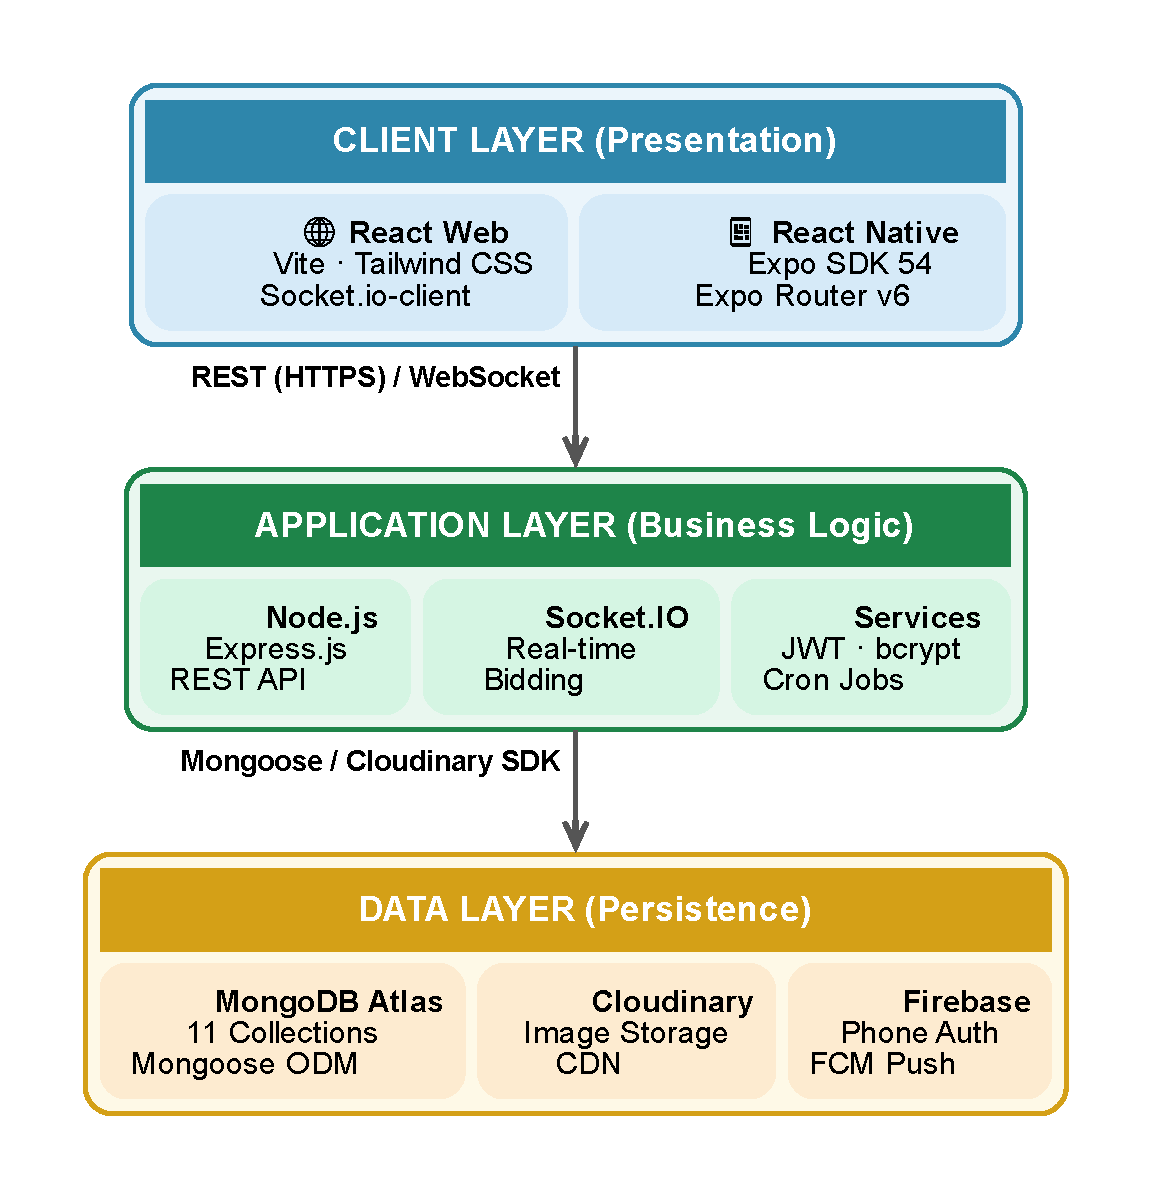
\includegraphics[width=0.85\textwidth]{3tier.pdf}
  \caption{3-tier архитектурын ерөнхий зураг}
  \label{fig:3tier}
\end{figure}

\subsection{Client давхарга (Presentation Layer)}

\begin{itemize}
  \item \textbf{Веб клиент} — React.js + Vite ашиглан хөгжүүлсэн SPA, responsive дизайнтай.
  \item \textbf{Мобайл клиент} — React Native + Expo ашиглан хөгжүүлсэн cross-platform мобайл апп.
  \item \textbf{Харилцааны протокол} — RESTful API (HTTPS) болон WebSocket (Socket.IO).
\end{itemize}

\subsection{Бизнес логикийн давхарга (Application Layer)}

Backend API нь дараах функцүүдийг агуулна:
\begin{itemize}
  \item Хэрэглэгчийн баталгаажуулалт (JWT, Google OAuth, Firebase Phone Auth)
  \item Бараа удирдах (CRUD үйлдлүүд, зураг хадгалалт)
  \item Дуудлага худалдааны логик (санал авах, статус шалгах)
  \item Бодит цагийн мэдээлэл дамжуулалт (Socket.IO room broadcast)
  \item Cron job-ууд (дуудлага дуусгах, ялагч тогтоох)
\end{itemize}

\subsection{Socket.IO Event загвар}

\begin{table}[H]
  \centering
  \caption{Socket.IO үндсэн event-үүд}
  \label{tab:socket-events}
  \begin{tabularx}{\textwidth}{L{4.5cm}L{3cm}L{6.5cm}}
    \toprule
    \textbf{Event} & \textbf{Чиглэл} & \textbf{Тайлбар} \\
    \midrule
    \texttt{joinAuction(productId)} & Client → Server & Дуудлагын room-д орох \\
    \texttt{leaveAuction(productId)} & Client → Server & Room-оос гарах \\
    \texttt{placeBid(\{productId, amount\})} & Client → Server & Шинэ үнэ санал \\
    \texttt{bidUpdate(\{productId, currentBid\})} & Server → Room & Бүх оролцогчид шинэ үнэ зарлах \\
    \texttt{auctionEnded(\{productId, winnerId\})} & Server → Room & Дуудлага дуусгасан \\
    \texttt{outbid(\{productId, newBid\})} & Server → User & Гүйцсэн мэдэгдэл \\
    \texttt{notification(\{type, message\})} & Server → User & Push-маягийн мэдэгдэл \\
    \bottomrule
  \end{tabularx}
\end{table}

\section{Use Case тайлбар}

\subsection{Use Case 1: Бараа байршуулах}

\begin{itemize}
  \item \textbf{Actor}: Бүртгэлтэй хэрэглэгч
  \item \textbf{Main flow}: Гарчиг, тайлбар, ангилал, нөхцөл, зураг оруулна → AI ангилал санал болгоно → Дуудлагын тохиргоо тавина → Хадгалдаг → Зургийг Cloudinary дээр upload, мэдээллийг MongoDB-д хадгална.
  \item \textbf{Alternative}: Зураг 20-оос их → алдаа буцаах.
\end{itemize}

\subsection{Use Case 2: Дуудлагад оролцох (place bid)}

\begin{itemize}
  \item \textbf{Main flow}: \texttt{joinAuction} event → Үнэ оруулах → Server нь баланс, currentBid шалгана → Bidding баримт үүсгэх → \texttt{bidUpdate} broadcast → Өмнөх highestBidder-д \texttt{outbid} + push notification.
  \item \textbf{Alternative}: Хангалтгүй balance → 400 "Insufficient balance".
\end{itemize}

\subsection{Use Case 3: Дуудлага дуусах (System)}

\begin{itemize}
  \item \textbf{Trigger}: Cron job — \texttt{bidDeadline <= Date.now()}
  \item \textbf{Main flow}: Auction-ыг \texttt{ended} болгоно → Хамгийн өндөр санал өгсөн хэрэглэгчийг \texttt{soldTo} болгоно → Buyer-ийн balance-аас үнийг хасна → Seller-ийн balance-д нэмнэ → Transaction баримт үүсгэнэ → Мэдэгдэл явуулна.
\end{itemize}

\section{ERD (Entity Relation Diagram)}

\begin{figure}[H]
  \centering
  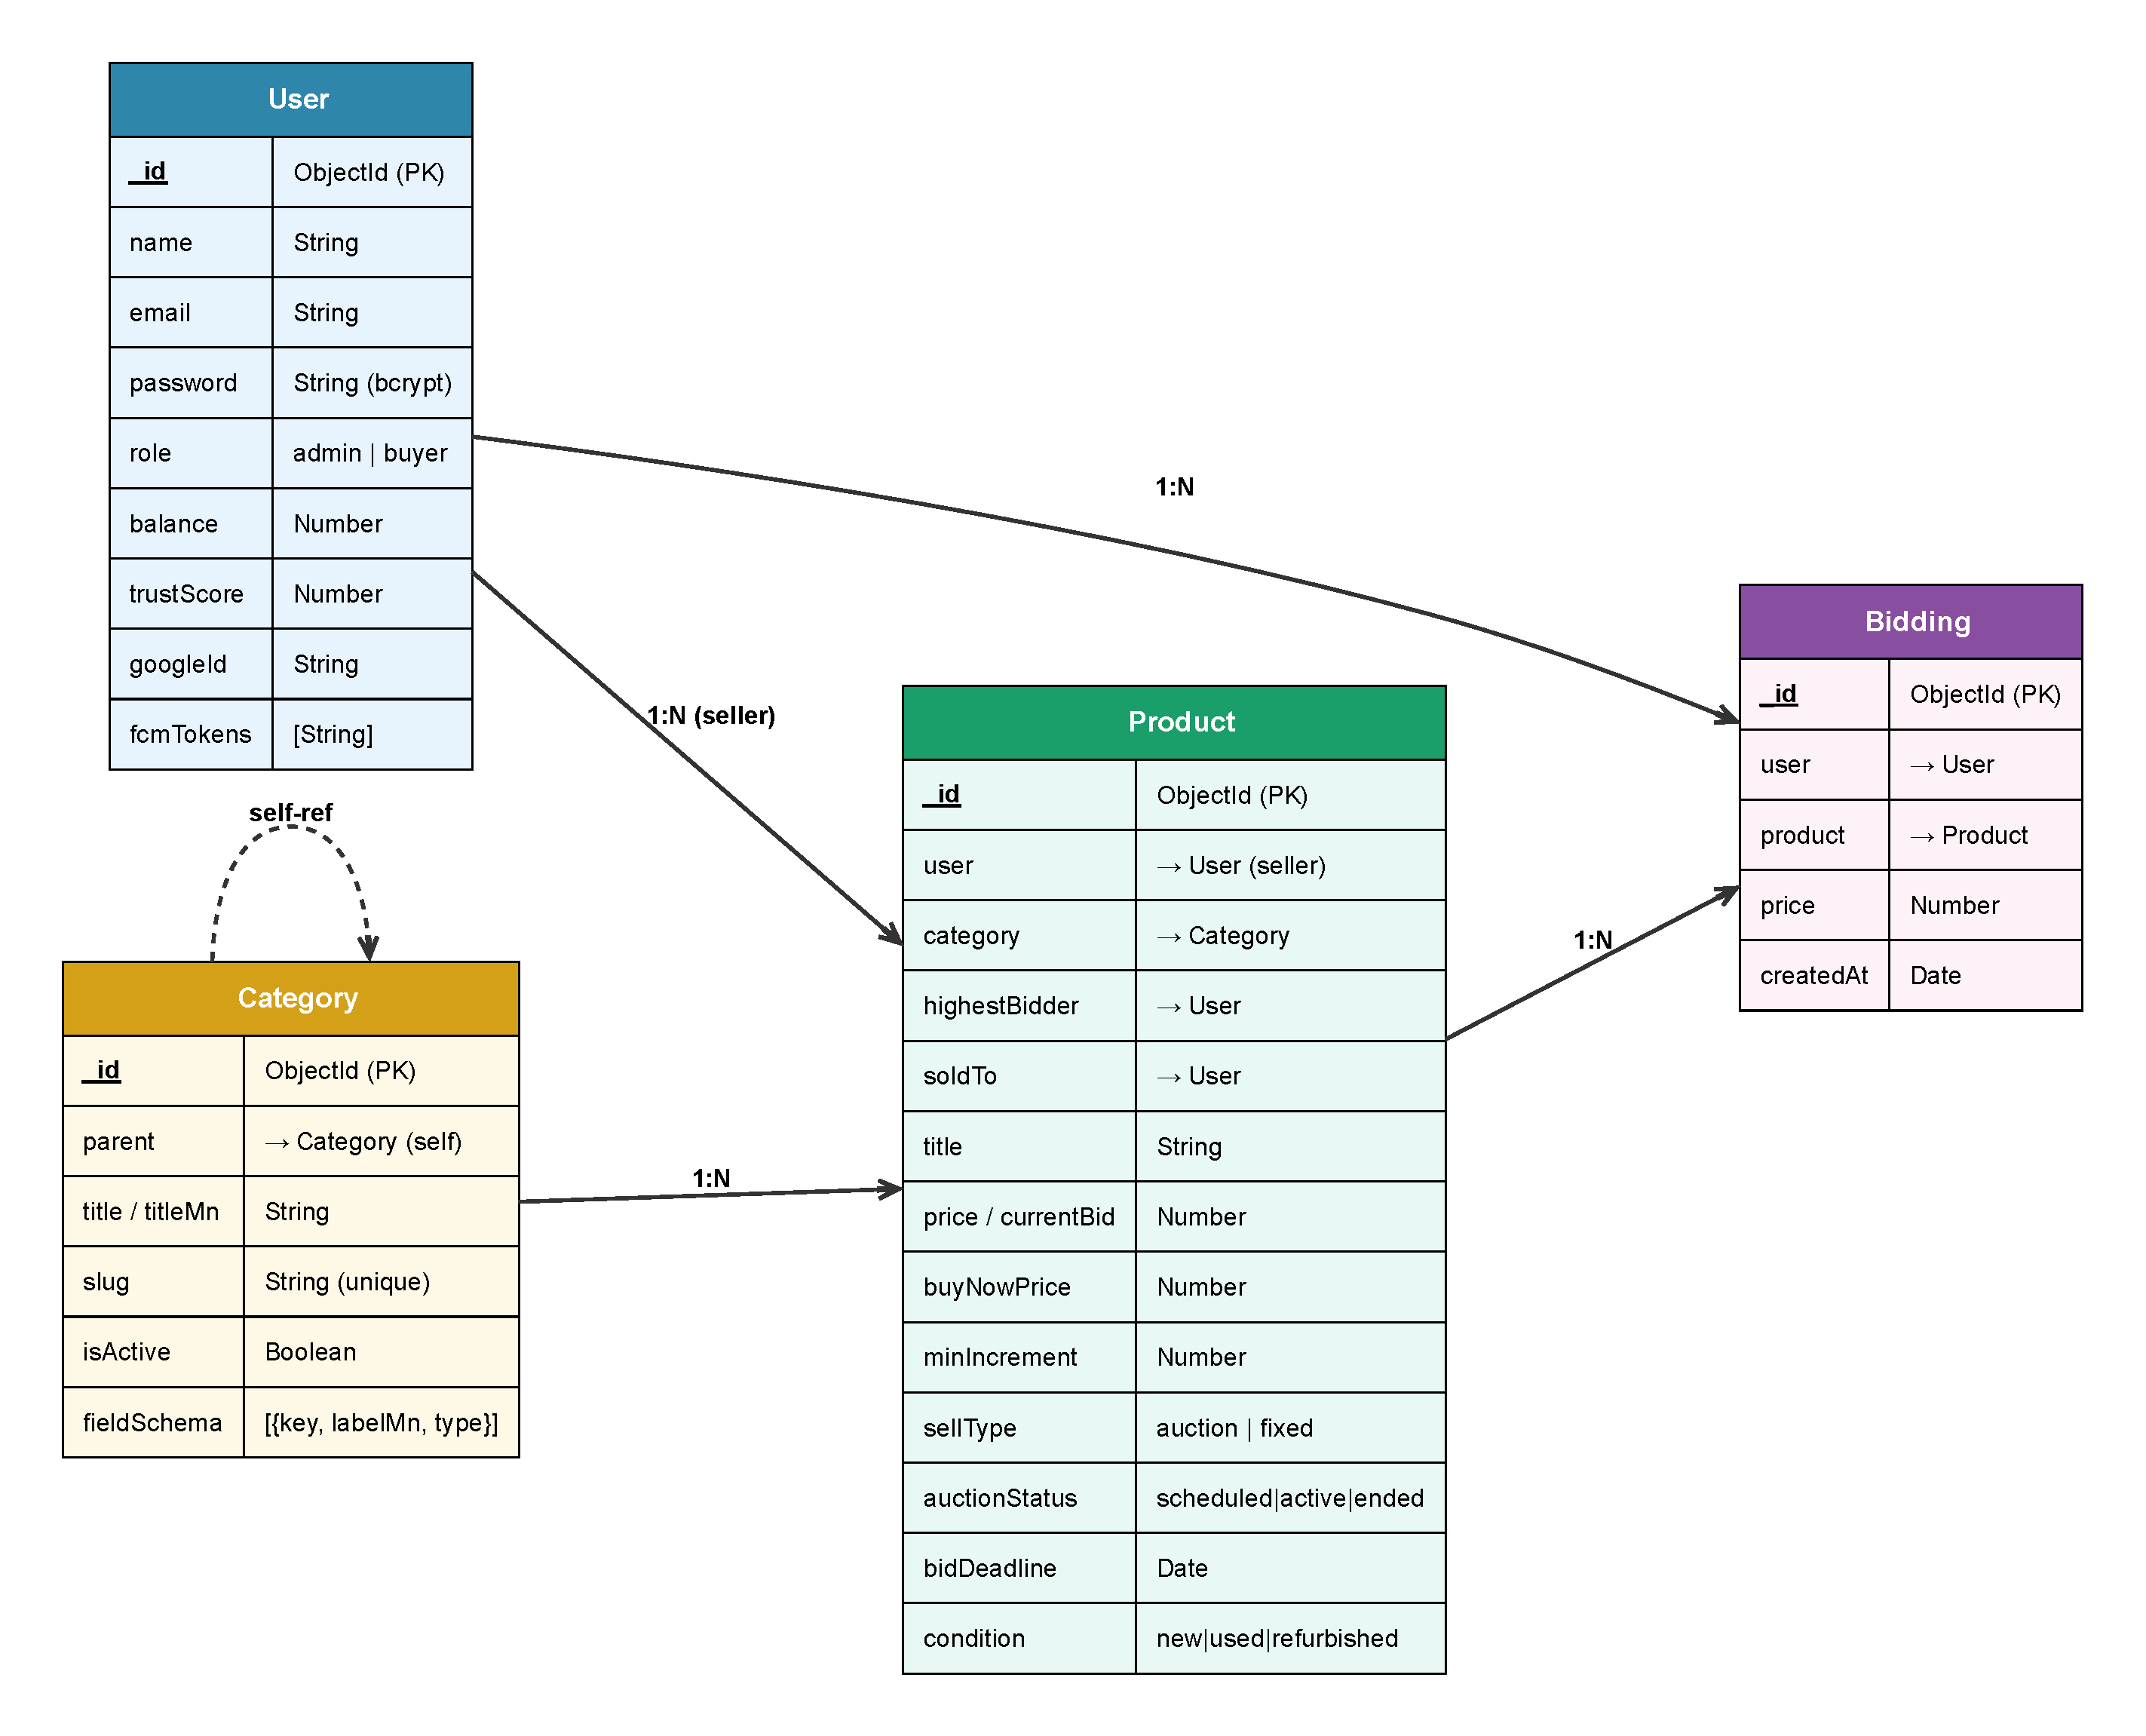
\includegraphics[width=\textwidth]{erd_core.pdf}
  \caption{Үндсэн entity-үүдийн хамаарал: User, Product, Category, Bidding}
  \label{fig:erd-core}
\end{figure}

\begin{figure}[H]
  \centering
  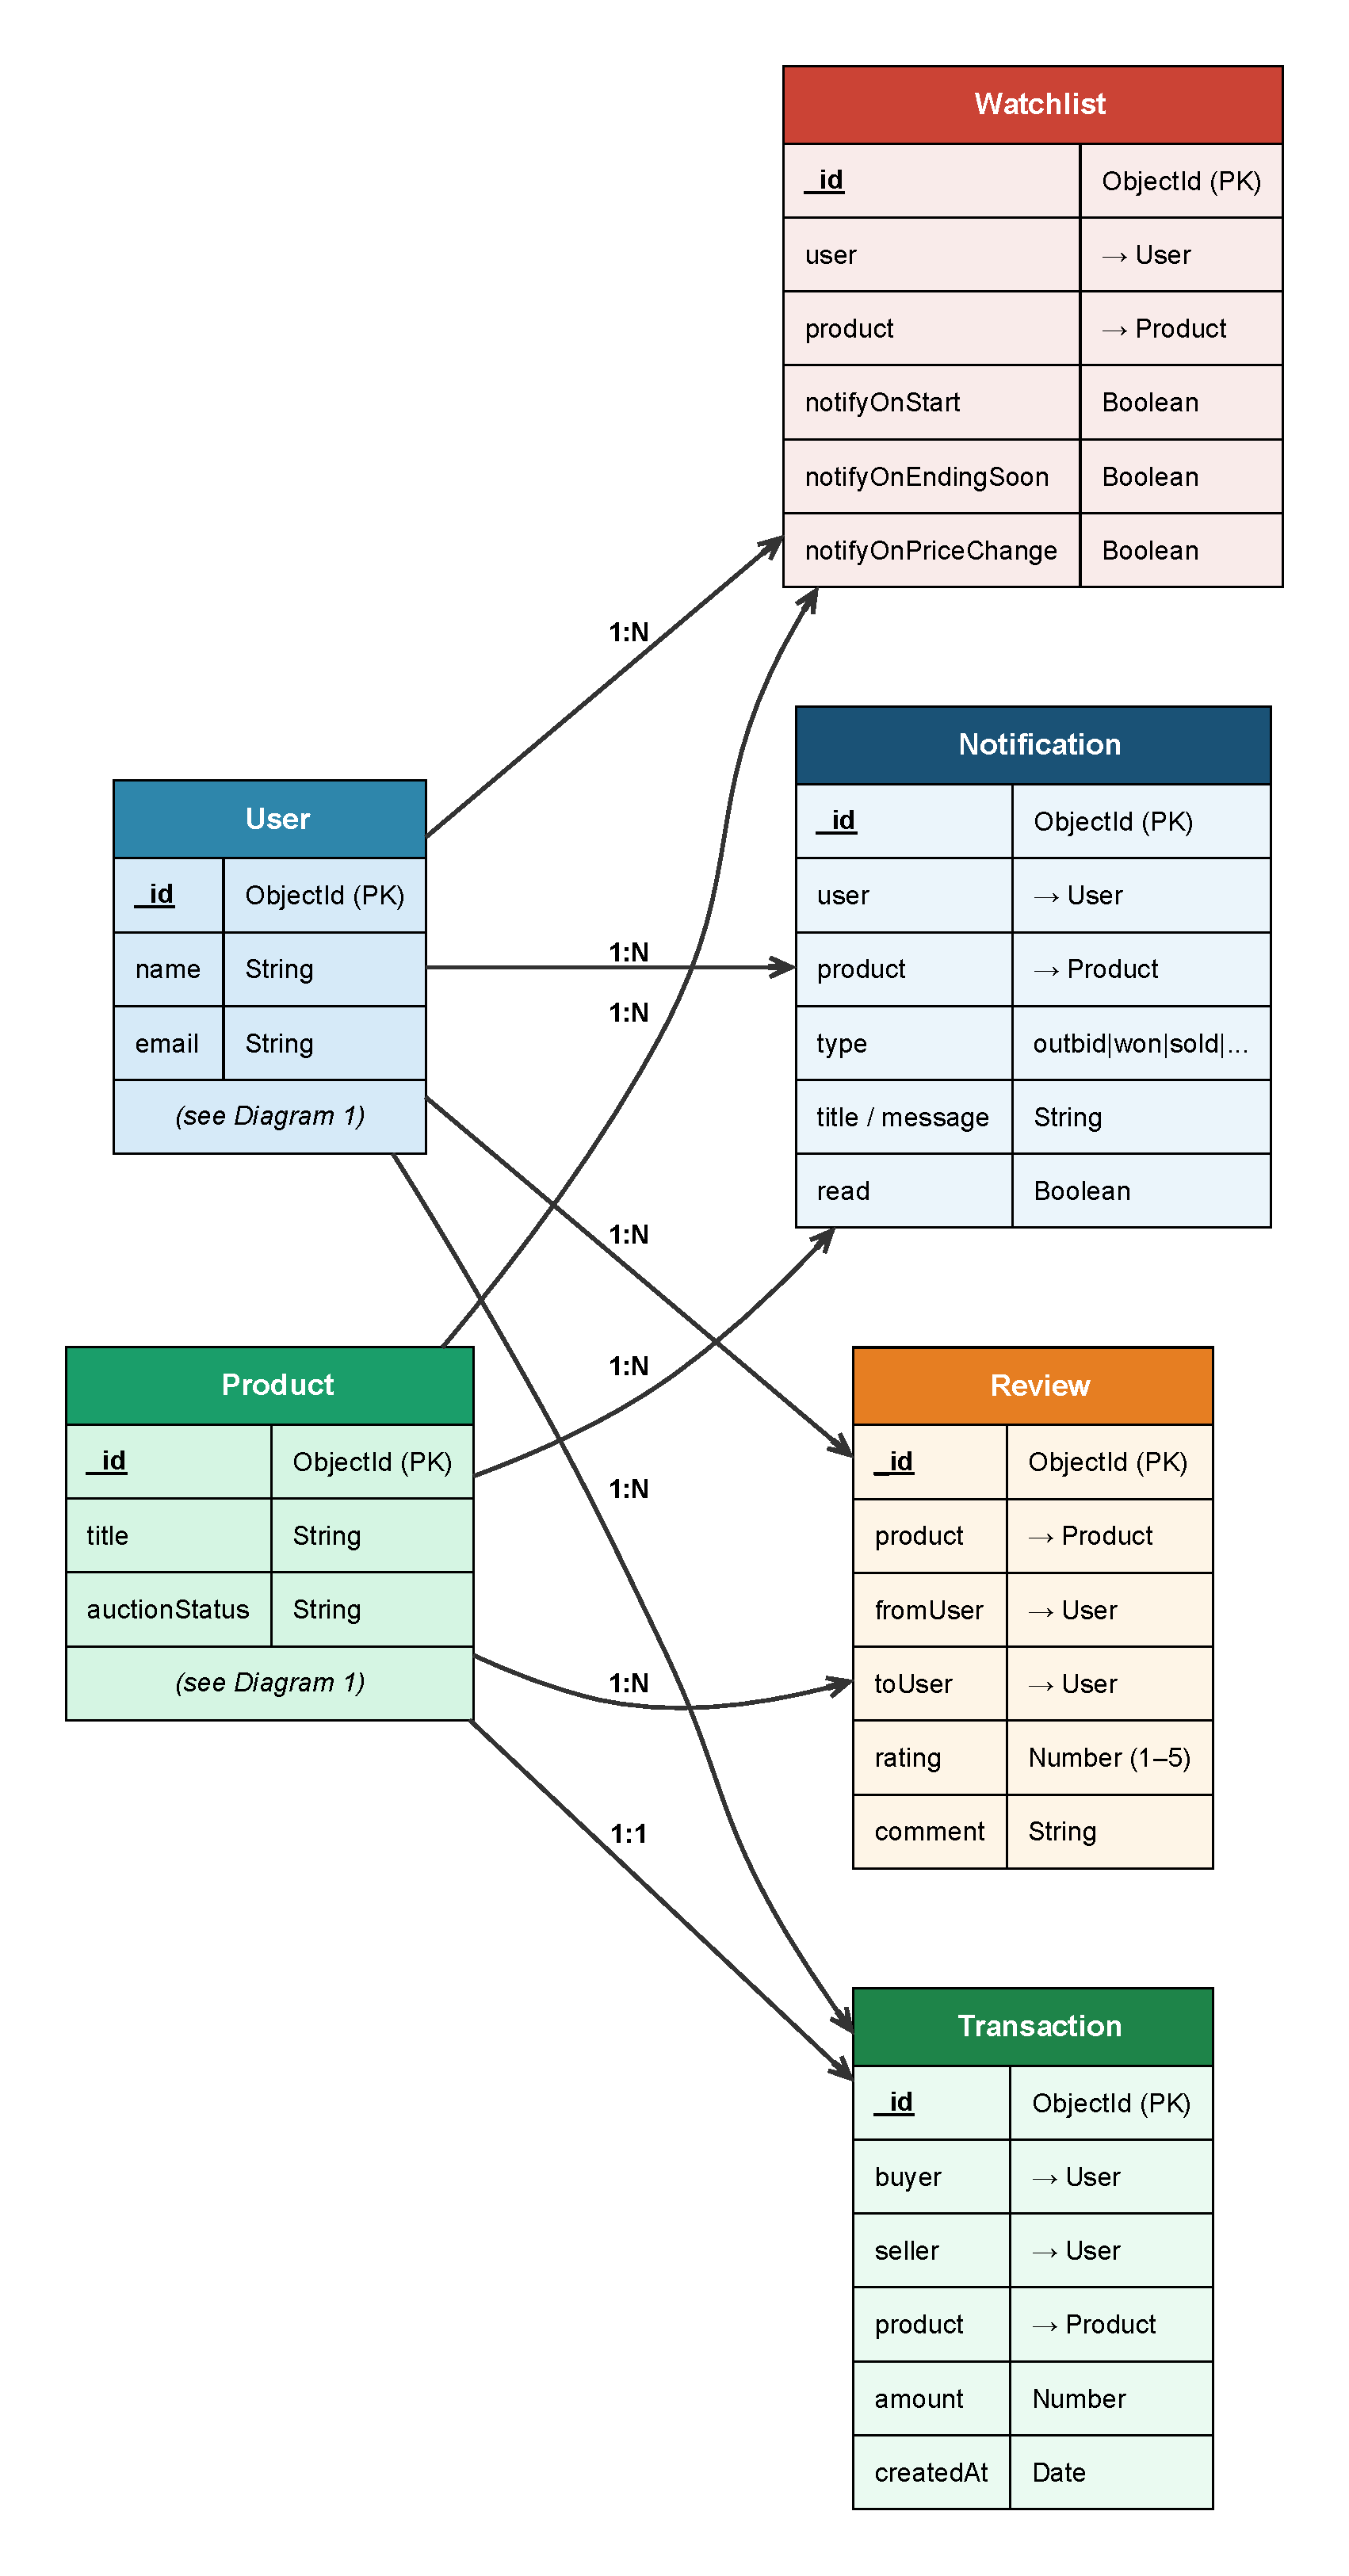
\includegraphics[width=\textwidth, height=0.82\textheight, keepaspectratio]{erd_support.pdf}
  \caption{Туслах entity-үүдийн хамаарал: Watchlist, Transaction, Review, Notification}
  \label{fig:erd-support}
\end{figure}

Системийн өгөгдлийн сан нь MongoDB ашигладаг бөгөөд 11 үндсэн collection-той.

\begin{table}[H]
  \centering
  \caption{Үндсэн entity-ийн хамаарлууд}
  \label{tab:entity-relations}
  \begin{tabularx}{\textwidth}{L{2.5cm}L{2.5cm}C{2.5cm}L{5cm}}
    \toprule
    \textbf{From} & \textbf{To} & \textbf{Cardinality} & \textbf{Тайлбар} \\
    \midrule
    User & Product & 1:N (seller) & Нэг хэрэглэгч олон бараа байршуулна \\
    User & Bidding & 1:N (bidder) & Хэрэглэгч олон bid өгнө \\
    Product & Bidding & 1:N & Нэг бараа олон bid авна \\
    Product & Watchlist & 1:N & Олон хэрэглэгч ажиглана \\
    Category & Category & 1:N (parent) & Hierarchy \\
    Category & Product & 1:N & Ангилалд олон бараа \\
    User & Transaction & 1:N (buyer/seller) & Гүйлгээний хамаарал \\
    \bottomrule
  \end{tabularx}
\end{table}

\section{Өгөгдлийн загвар дэлгэрэнгүй}

\subsection{User Collection}

User collection нь системийн төв entity бөгөөд authentication-ийн бүх хувилбарыг нэг баримтад нэгтгэдэг. Чухал талбарууд:

\begin{itemize}
  \item \texttt{email, password (bcrypt hash), phone, phoneVerified}
  \item \texttt{role: 'admin' | 'buyer'}
  \item \texttt{balance} — Дотоод данс (төгрөгөөр)
  \item \texttt{fcmTokens [String]} — Push notification token-ууд
  \item \texttt{trustScore} — 0--100 хооронд; \texttt{completedDeals * 5 - cancelledBids * 10}-аар тооцоолно
  \item \texttt{googleId, eMongoliaId, eMongoliaVerified}
\end{itemize}

\subsection{Product Collection}

Auction-д тавьсан барааг агуулна. Чухал талбарууд:

\begin{itemize}
  \item \textbf{Үнийн загвар}: \texttt{price} (starting), \texttt{currentBid}, \texttt{reservePrice}, \texttt{buyNowPrice}, \texttt{minIncrement}
  \item \textbf{Auction lifecycle}: \texttt{startMode}, \texttt{auctionStart}, \texttt{bidDeadline}, \texttt{auctionStatus} (scheduled | active | ended)
  \item \textbf{Машины тусгай}: \texttt{vin, make, model, year, mileage, fuelType}
\end{itemize}

\subsection{Bidding Collection}

Өчүүхэн жижиг schema-тай боловч хамгийн өндөр write-нагрузка авдаг. Индекс: \texttt{\{ product: 1, price: -1, createdAt: -1 \}} — bid history-ийг үнээр буурах эрэмбээр шуурхай авах боломж.

\section{API дизайны зарчим}

\begin{itemize}
  \item \textbf{RESTful} — Resource-based URL, HTTP method-ыг семантикаар ашиглах.
  \item \textbf{Error format} — \texttt{\{ error: 'message', code: 'ERR\_CODE' \}}
  \item \textbf{Status codes} — 200, 201, 400, 401, 403, 404, 422, 429, 500.
  \item \textbf{Pagination} — \texttt{?page=1\&limit=20}, response-д \texttt{total, page, hasMore}.
\end{itemize}

\section{Бүлгийн дүгнэлт}

Энэ бүлэгт системийн актеруудыг тодорхойлж, функциональ ба функциональ бус шаардлагуудыг нарийвчилсан. 3-tier архитектурын үндэслэлийг тайлбарлаж, Socket.IO event загвар, REST API дизайны зарчмыг тогтоосон. 11 collection-той MongoDB загварыг гаргасан.

% =====================================================================
%  CHAPTER 3 — IMPLEMENTATION
% =====================================================================
\chapter{Системийн хөгжүүлэлт}

Энэхүү бүлэгт онлайн дуудлага худалдааны бүрэн цогц системийн хөгжүүлэлтийн талаар дэлгэрэнгүй тайлбарлана. Систем нь 3 үндсэн бүрэлдэхүүн хэсгээс бүрдэнэ: (1) \textbf{Backend API}, (2) \textbf{Веб аппликейшн}, (3) \textbf{Мобайл аппликейшн}.

Хөгжүүлэлт нийт \textasciitilde12,000 мөр кодтой: backend \textasciitilde4,500, frontend \textasciitilde3,500, mobile \textasciitilde4,000.

\section{Хөгжүүлэлтийн орчин}

\begin{itemize}
  \item OS: Windows 11 + WSL2 (Ubuntu 22.04)
  \item Editor: VS Code with ESLint, Prettier
  \item Node.js v20 LTS, \texttt{nodemon} dev, \texttt{pm2} production
  \item Git: GitHub repository, \texttt{main} + \texttt{develop} branch model
\end{itemize}

\section{Системийн модулиуд}

\subsection{User Module}

\begin{itemize}
  \item \texttt{models/User.js} — bcrypt password hash, JWT token методууд.
  \item \texttt{controllers/userController.js} — \texttt{register}, \texttt{login}, \texttt{forgotPassword}, \texttt{resetPassword}, \texttt{verifyEmail}, \texttt{addBalance}, \texttt{getProfile}, \texttt{updatePhoto}.
  \item \texttt{services/emailService.js} — Nodemailer ашиглан SMTP-ээр и-мэйл.
  \item \texttt{services/googleAuthService.js} — Google OAuth verification.
\end{itemize}

\subsection{Product Module}

\begin{itemize}
  \item \texttt{models/Product.js} — Барааны schema, олон тооны талбар, машины тусгай талбаруудыг агуулсан.
  \item \texttt{controllers/productController.js} — CRUD + \texttt{suggestCategory}, \texttt{myActiveAuctions}.
  \item \texttt{services/categoryAiService.js} — Baraaны title/description-аас тохирох ангилал санал болгох.
\end{itemize}

\subsection{Bidding Module}

Үндсэн логик (псевдо код):

\begin{lstlisting}[caption={Bid placement логик}, label={lst:placebid}]
async function placeBid(req, res) {
  const { productId, amount } = req.body;

  // 1. Product status check
  const product = await Product.findById(productId);
  if (product.auctionStatus !== 'active')
    return error(400, 'Auction not active');

  // 2. Minimum increment check
  const minNext = product.currentBid + product.minIncrement;
  if (amount < minNext) return error(400, `Bid >= ${minNext}`);

  // 3. Balance check
  const user = await User.findById(userId);
  if (user.balance < amount)
    return error(400, 'Insufficient balance');

  // 4. Atomic transaction
  const session = await mongoose.startSession();
  session.startTransaction();
  try {
    await Bidding.create([{ user: userId, product: productId,
      price: amount }], { session });
    product.currentBid = amount;
    product.highestBidder = userId;
    await product.save({ session });
    await session.commitTransaction();

    // 5. Real-time broadcast
    io.to(`auction:${productId}`).emit('bidUpdate', {
      productId, currentBid: amount, highestBidder: userId
    });

    // 6. Outbid notification
    if (prevHighestBidder) {
      io.to(`user:${prevHighestBidder}`).emit('outbid', { productId });
      sendFCM(prevHighestBidder, { title: 'Гүйцсэн!', body: '...' });
    }
    res.status(201).json({ bid });
  } catch (e) {
    await session.abortTransaction(); throw e;
  } finally { session.endSession(); }
}
\end{lstlisting}

\subsection{Auction Lifecycle Cron Job}

\texttt{cron/auctionCloser.js} нь 1 минут тутамд ажиллаж:
\begin{itemize}
  \item Scheduled auctions-аас \texttt{auctionStart <= now} бүгдийг \texttt{active} болгоно.
  \item Active auctions-аас \texttt{bidDeadline <= now} бүгдийг \texttt{ended} болгоно.
  \item \texttt{highestBidder} байгаа бол \texttt{soldTo}-г тогтоож, balance шилжүүлж, Transaction үүсгэнэ.
  \item Ялагч + ялагдагсадад мэдэгдэл явуулна.
\end{itemize}

\section{API болон өгөгдөл солилцоо}

\subsection{Үндсэн endpoint бүлэг}

\begin{table}[H]
  \centering
  \caption{Системийн үндсэн API endpoint-ууд}
  \label{tab:api-endpoints}
  \begin{tabularx}{\textwidth}{L{3.5cm}L{8.5cm}}
    \toprule
    \textbf{Бүлэг} & \textbf{Endpoint-ууд} \\
    \midrule
    \texttt{/api/users} & register, login, logout, allusers, userbalance, google \\
    \texttt{/api/product} & products, create, :id, my, my/active, suggest-category \\
    \texttt{/api/bidding} & place, :productId, my, my-wins, my-losses \\
    \texttt{/api/request} & create invoice, poll status, my history \\
    \texttt{/api/category} & CRUD + hierarchy \\
    \texttt{/api/watchlist} & add, remove, list \\
    \texttt{/api/notifications} & list, unread-count, :id/read \\
    \texttt{/api/reviews} & create, product/:id, user/:id \\
    \texttt{/api/search} & global search with filters \\
    \texttt{/api/admin} & dashboard, statistics \\
    \texttt{/api/webhook} & qpay-webhook (public) \\
    \bottomrule
  \end{tabularx}
\end{table}

\subsection{API хариу формат}

Амжилттай хариу:
\begin{lstlisting}[language={}]
{ "data": {...}, "message": "Success" }
\end{lstlisting}

Алдааны хариу:
\begin{lstlisting}[language={}]
{ "error": "Message", "code": "INSUFFICIENT_BALANCE" }
\end{lstlisting}

\section{Веб аппликейшны хөгжүүлэлт}

\subsection{Folder бүтэц}

\begin{lstlisting}[language={}, caption={Frontend folder бүтэц}]
frontend/
+-- src/
|   +-- components/      # ProductCard, BidForm, Navbar...
|   +-- screen/          # Home, ProductDetail, Profile, Admin...
|   +-- context/         # AuthContext, SocketContext
|   +-- hooks/           # useAuth, useSocket, useDebounce
|   +-- config/          # api.js (Axios wrapper)
|   +-- i18n/            # mn.json, en.json (Mongolian/English)
|   +-- utils/           # formatters, validators
|   +-- App.jsx
+-- public/
+-- vite.config.js
\end{lstlisting}

\subsection{Socket.IO интеграц веб дээр}

\texttt{SocketContext} нь app-аас глобал socket connection-ийг хэвээр барина. ProductDetail хуудас mount үед \texttt{joinAuction(productId)} event илгээж, unmount үед \texttt{leaveAuction} ажиллана. \texttt{bidUpdate} event-д тулгуурлан \texttt{currentBid} state шинэчлэгдэж UI шууд update хийгддэг.

\begin{figure}[H]
  \centering
  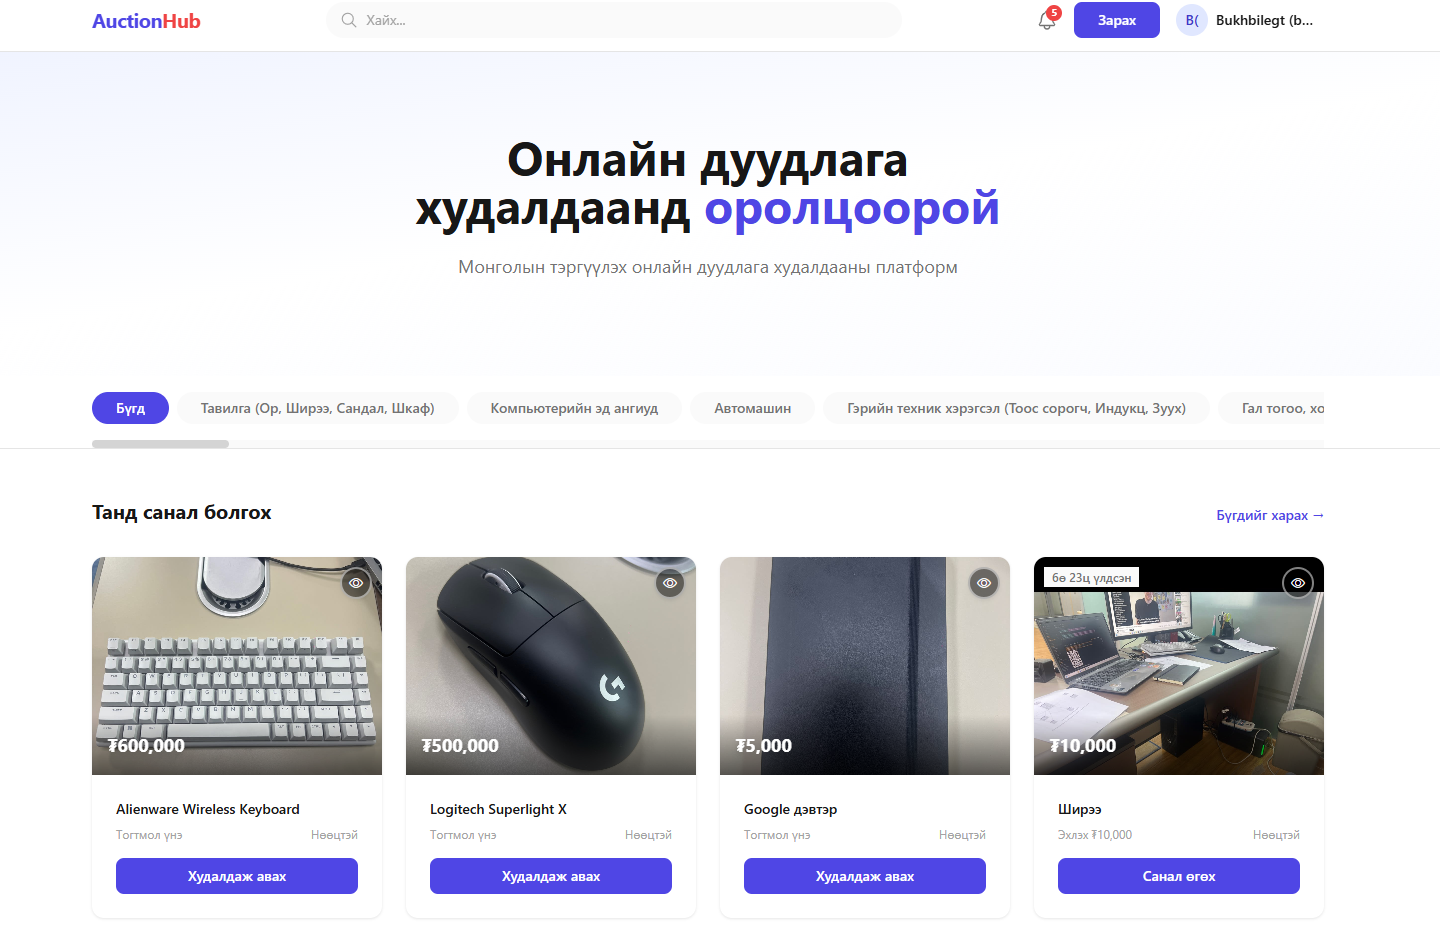
\includegraphics[width=\textwidth]{web_home.png}
  \caption{Веб аппликейшны нүүр хуудас — дуудлага худалдааны жагсаалт}
  \label{fig:web-home}
\end{figure}

\begin{figure}[H]
  \centering
  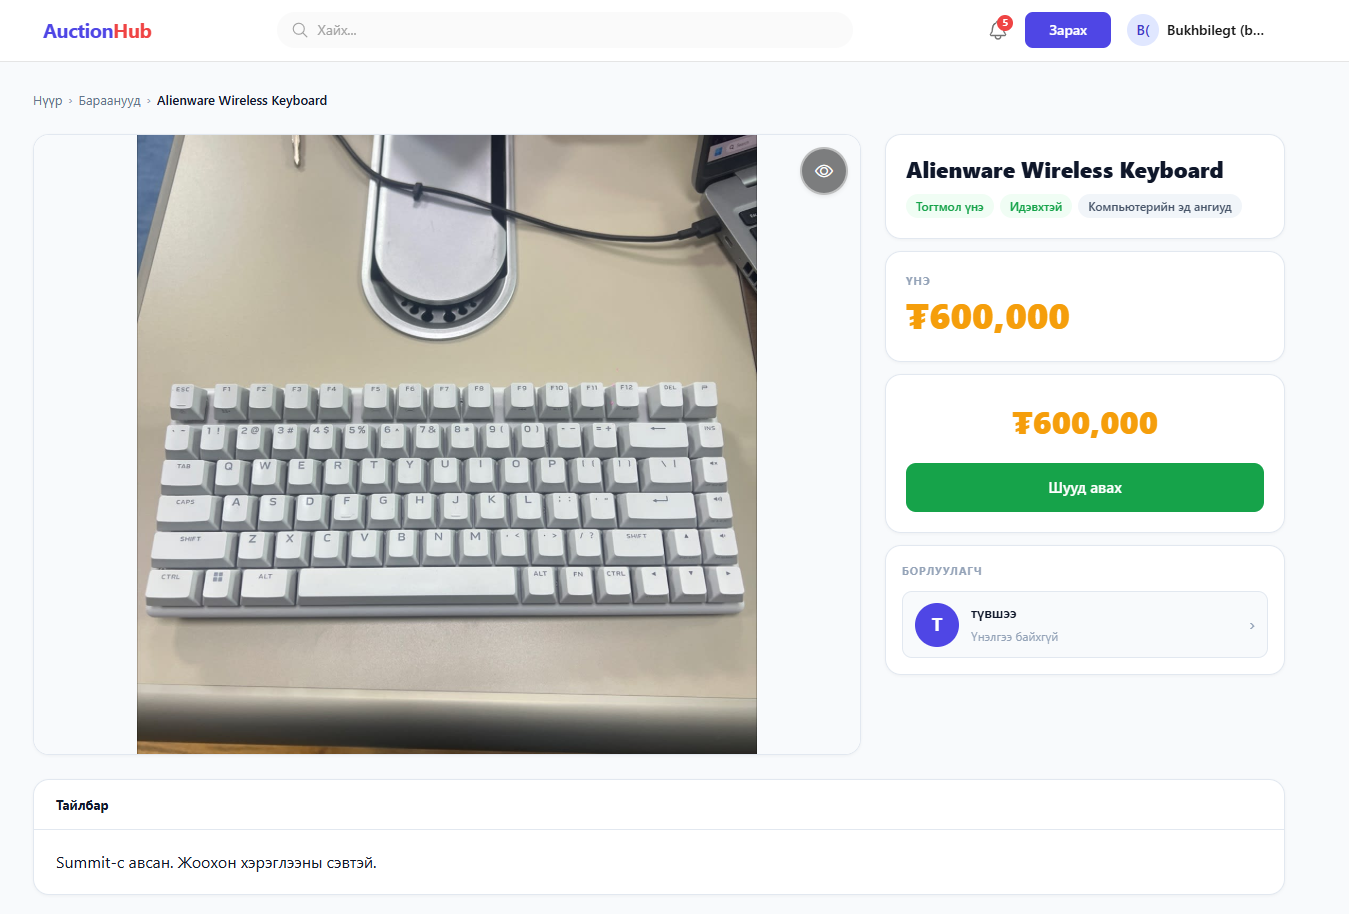
\includegraphics[width=0.85\textwidth]{web_product.png}
  \caption{Бараан дэлгэрэнгүй хуудас — шууд авах үнэ, дуудлагын мэдээлэл}
  \label{fig:web-product}
\end{figure}

\subsection{Админы dashboard}

\begin{itemize}
  \item \textbf{Хэрэглэгчид} — Жагсаалт, хайлт, түгжих/нээх, баланс цэнэглэх.
  \item \textbf{Бараа} — Бүх бараа, force-delete, verification badge олгох.
  \item \textbf{Ангилал} — CRUD + hierarchy editor.
  \item \textbf{Статистик} — Recharts ашиглан line/bar chart.
\end{itemize}

\begin{figure}[H]
  \centering
  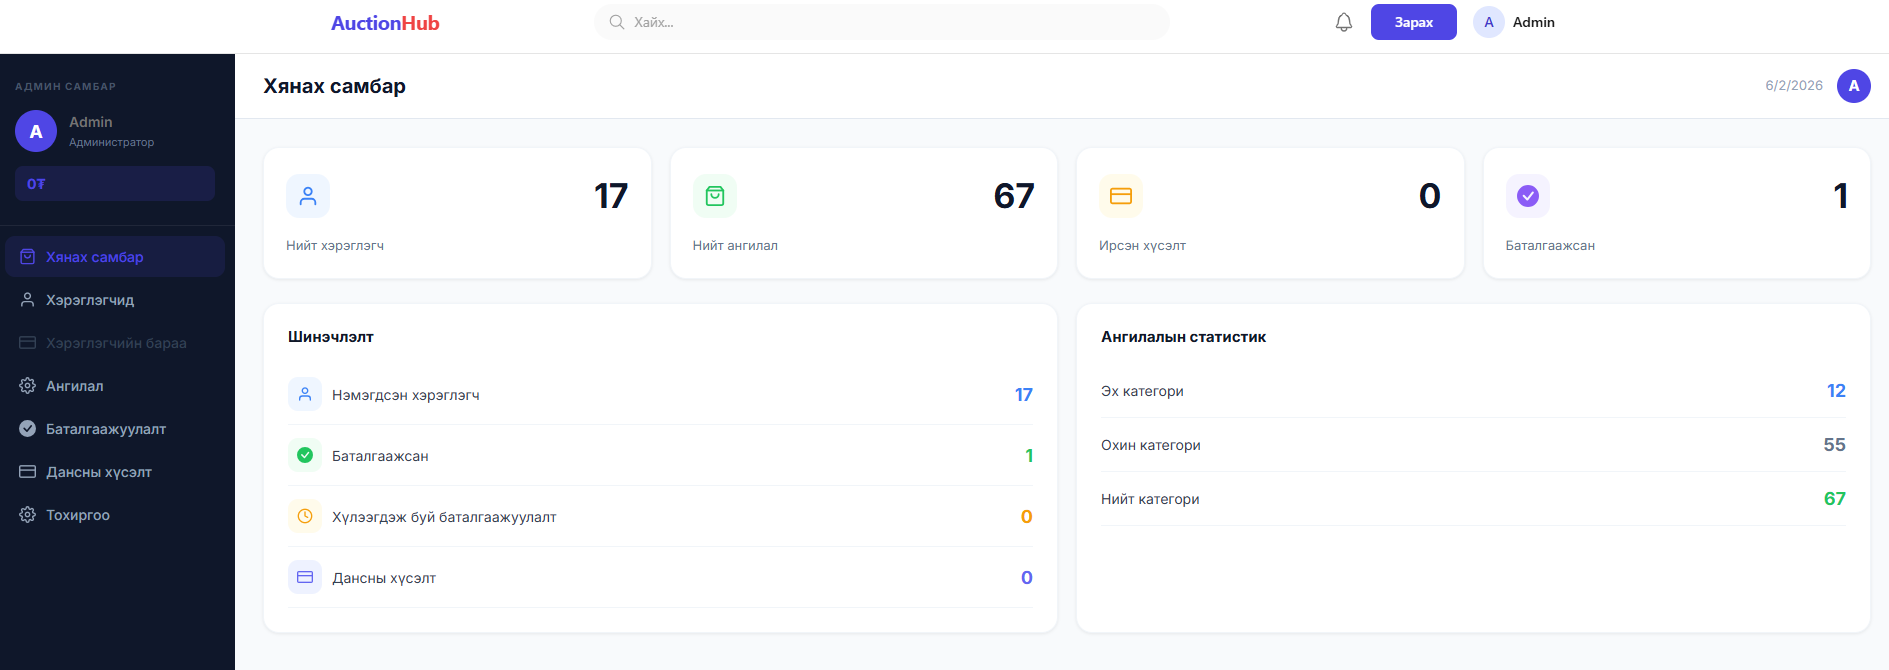
\includegraphics[width=\textwidth]{web_admin.png}
  \caption{Админы хянах самбар — хэрэглэгч, ангилал, баталгаажуулалтын статистик}
  \label{fig:web-admin}
\end{figure}

\subsection{Бараа нэмэх форм}

Хэрэглэгч бараа байршуулахдаа гарчиг, тайлбар, ангилал, зураг, үнэ, дуудлагын
хугацаа болон шууд зарагдах үнийг тохируулна. AI ангилал санал болгох, ноорог
автомат хадгалах функцуудтай.

\begin{figure}[H]
  \centering
  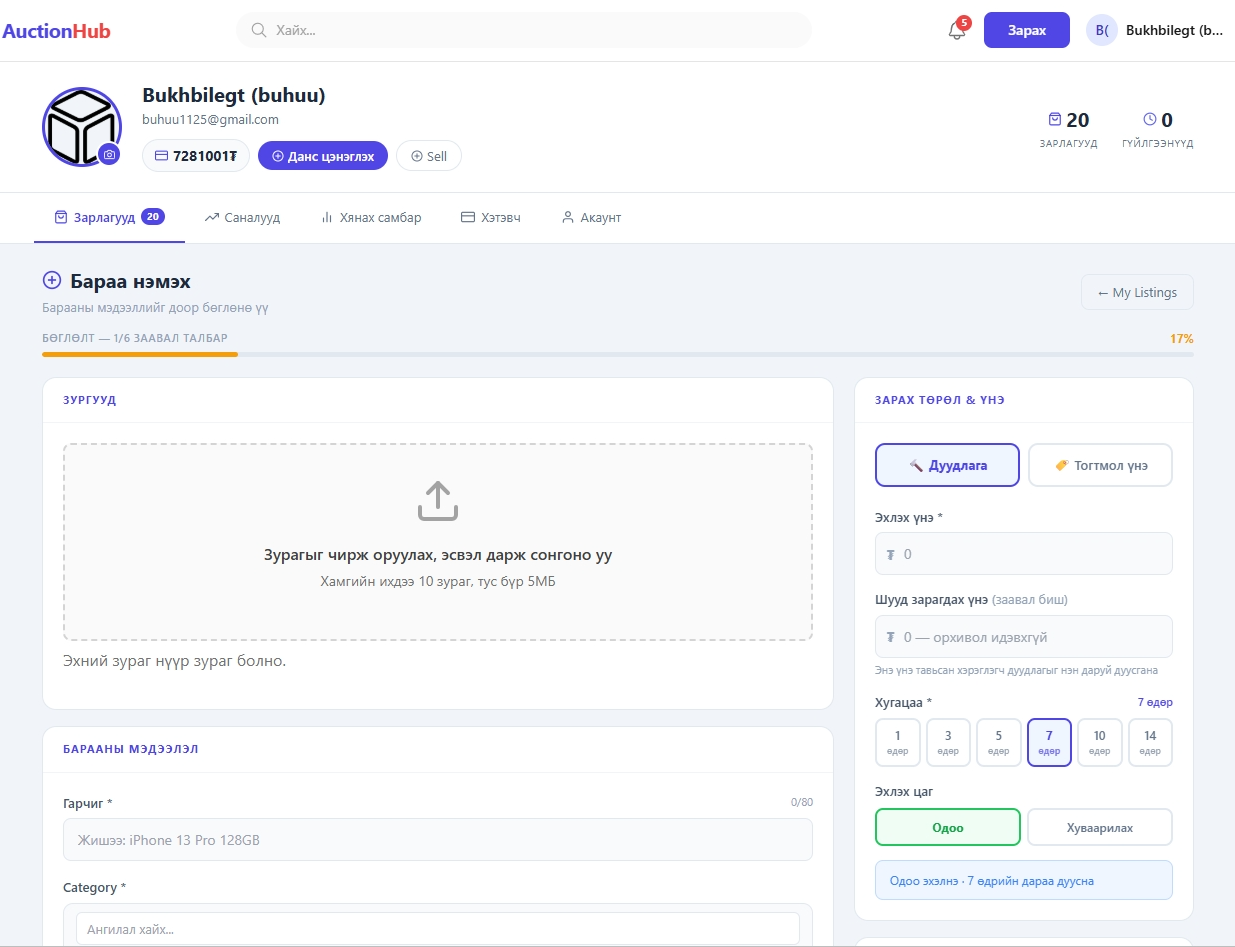
\includegraphics[width=\textwidth]{web_add_product1.png}
  \caption{Бараа нэмэх форм — зургийн upload, үнэ, хугацааны тохиргоо}
  \label{fig:web-add1}
\end{figure}

\begin{figure}[H]
  \centering
  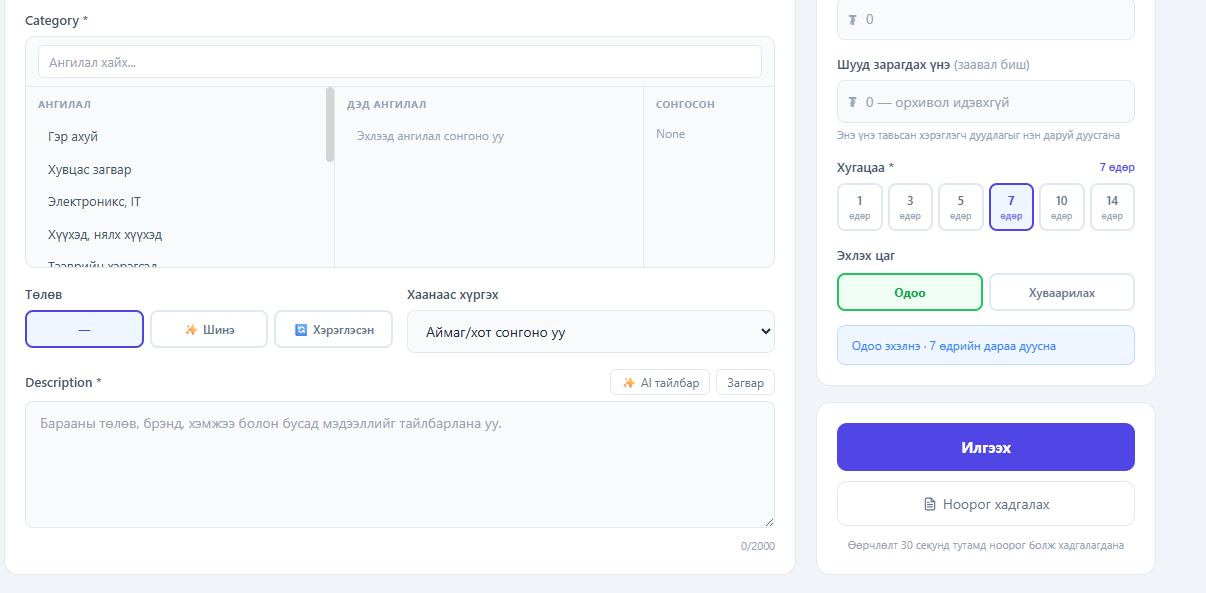
\includegraphics[width=\textwidth]{web_add_product2.png}
  \caption{Бараа нэмэх форм — ангилал сонгох, тайлбар, байрлал}
  \label{fig:web-add2}
\end{figure}

\subsection{Хэрэглэгчийн профайл}

\begin{figure}[H]
  \centering
  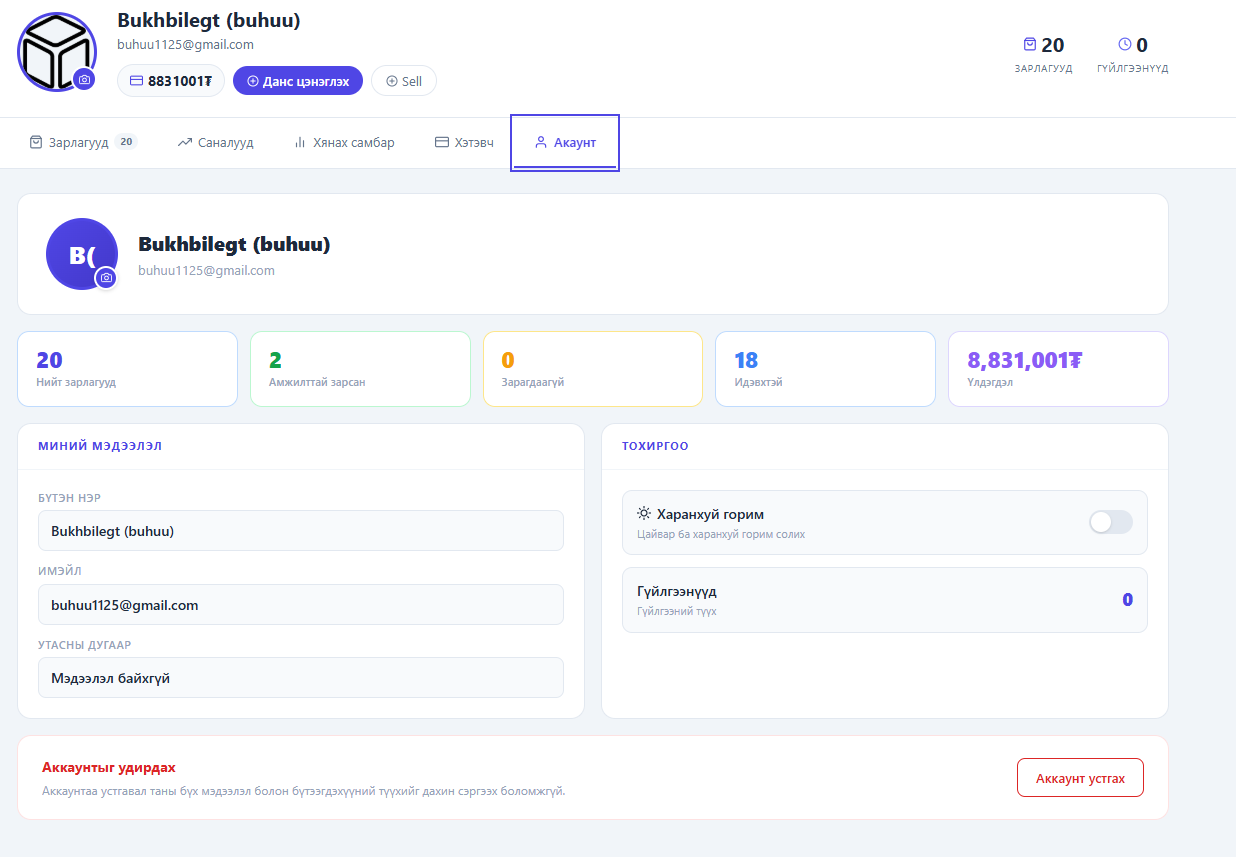
\includegraphics[width=\textwidth]{web_profile.png}
  \caption{Хэрэглэгчийн профайл — зарлагуud, баланс, тохиргоо}
  \label{fig:web-profile}
\end{figure}

\section{Мобайл аппликейшны хөгжүүлэлт}

\subsection{Folder бүтэц (Expo Router)}

\begin{lstlisting}[language={}, caption={Mobile folder бүтэц}]
mobile/auctionapp/
+-- app/
|   +-- (tabs)/
|   |   +-- index.tsx         # Home
|   |   +-- search.tsx
|   |   +-- selling.tsx
|   |   +-- notifications.tsx
|   |   +-- profile.tsx
|   +-- (hidden)/
|   |   +-- balance.tsx       # QPay payment screen
|   |   +-- login.tsx
|   |   +-- product/[id].tsx
|   +-- _layout.tsx
+-- components/
+-- hooks/
+-- lib/
+-- assets/
\end{lstlisting}

\subsection{Мобайл аппликейшны үндсэн функцууд}

\begin{itemize}
  \item \textbf{Баталгаажуулалт} — Google OAuth (Expo AuthSession), Firebase Phone Auth (SMS OTP), JWT + AsyncStorage.
  \item \textbf{Бараа удирдах} — expo-image-picker-ээр зураг, AI category, DateTimePicker.
  \item \textbf{Дуудлага худалдаа} — Socket.IO real-time, countdown таймер, үнийн түүхийн график.
  \item \textbf{QPay} — Дансны цэнэглэлтийн хуудас: дүн оруулах → QR харуулах → банкны апп deep link → 3 секунд тутам polling.
\end{itemize}

% ── Main screens ──────────────────────────────────────────────────────
\begin{figure}[H]
  \centering
  \begin{minipage}{0.45\textwidth}
    \centering
    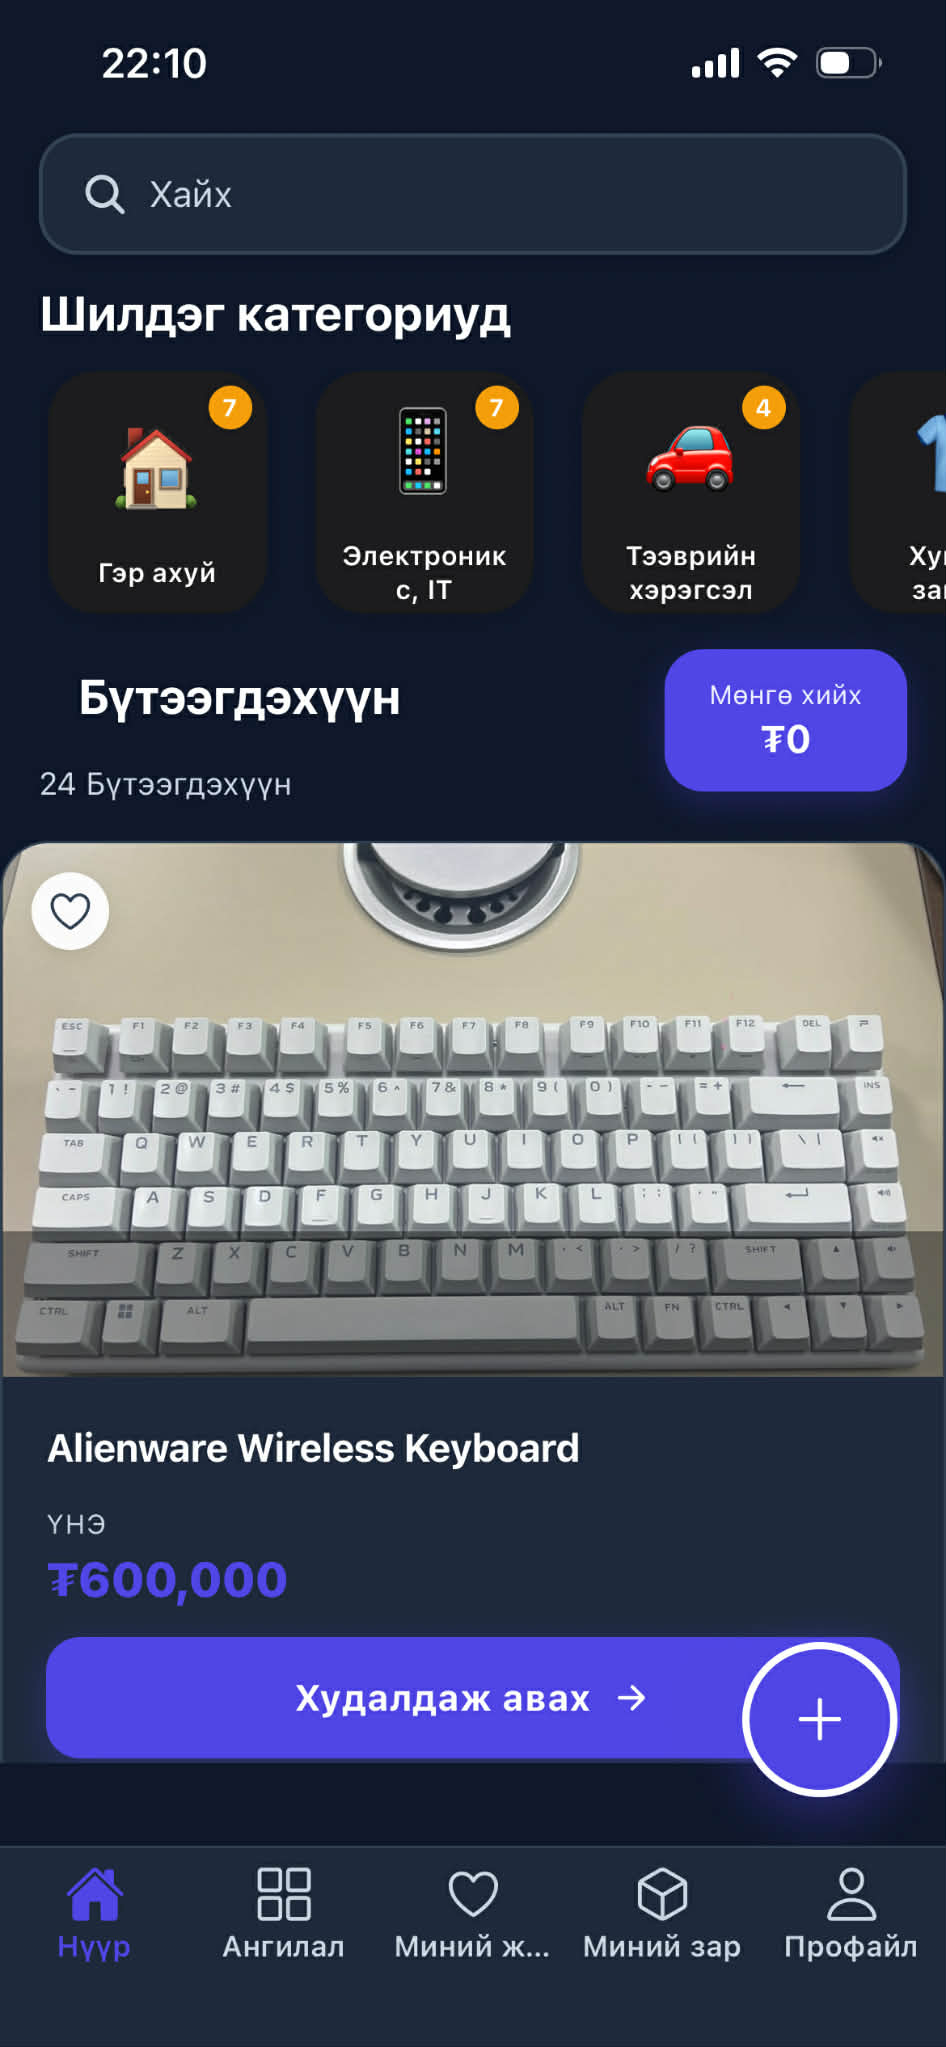
\includegraphics[width=\textwidth]{mobile_home.jpg}
    \caption{Нүүр хуудас — категори, бараан жагсаалт}
    \label{fig:mobile-home}
  \end{minipage}
  \hfill
  \begin{minipage}{0.45\textwidth}
    \centering
    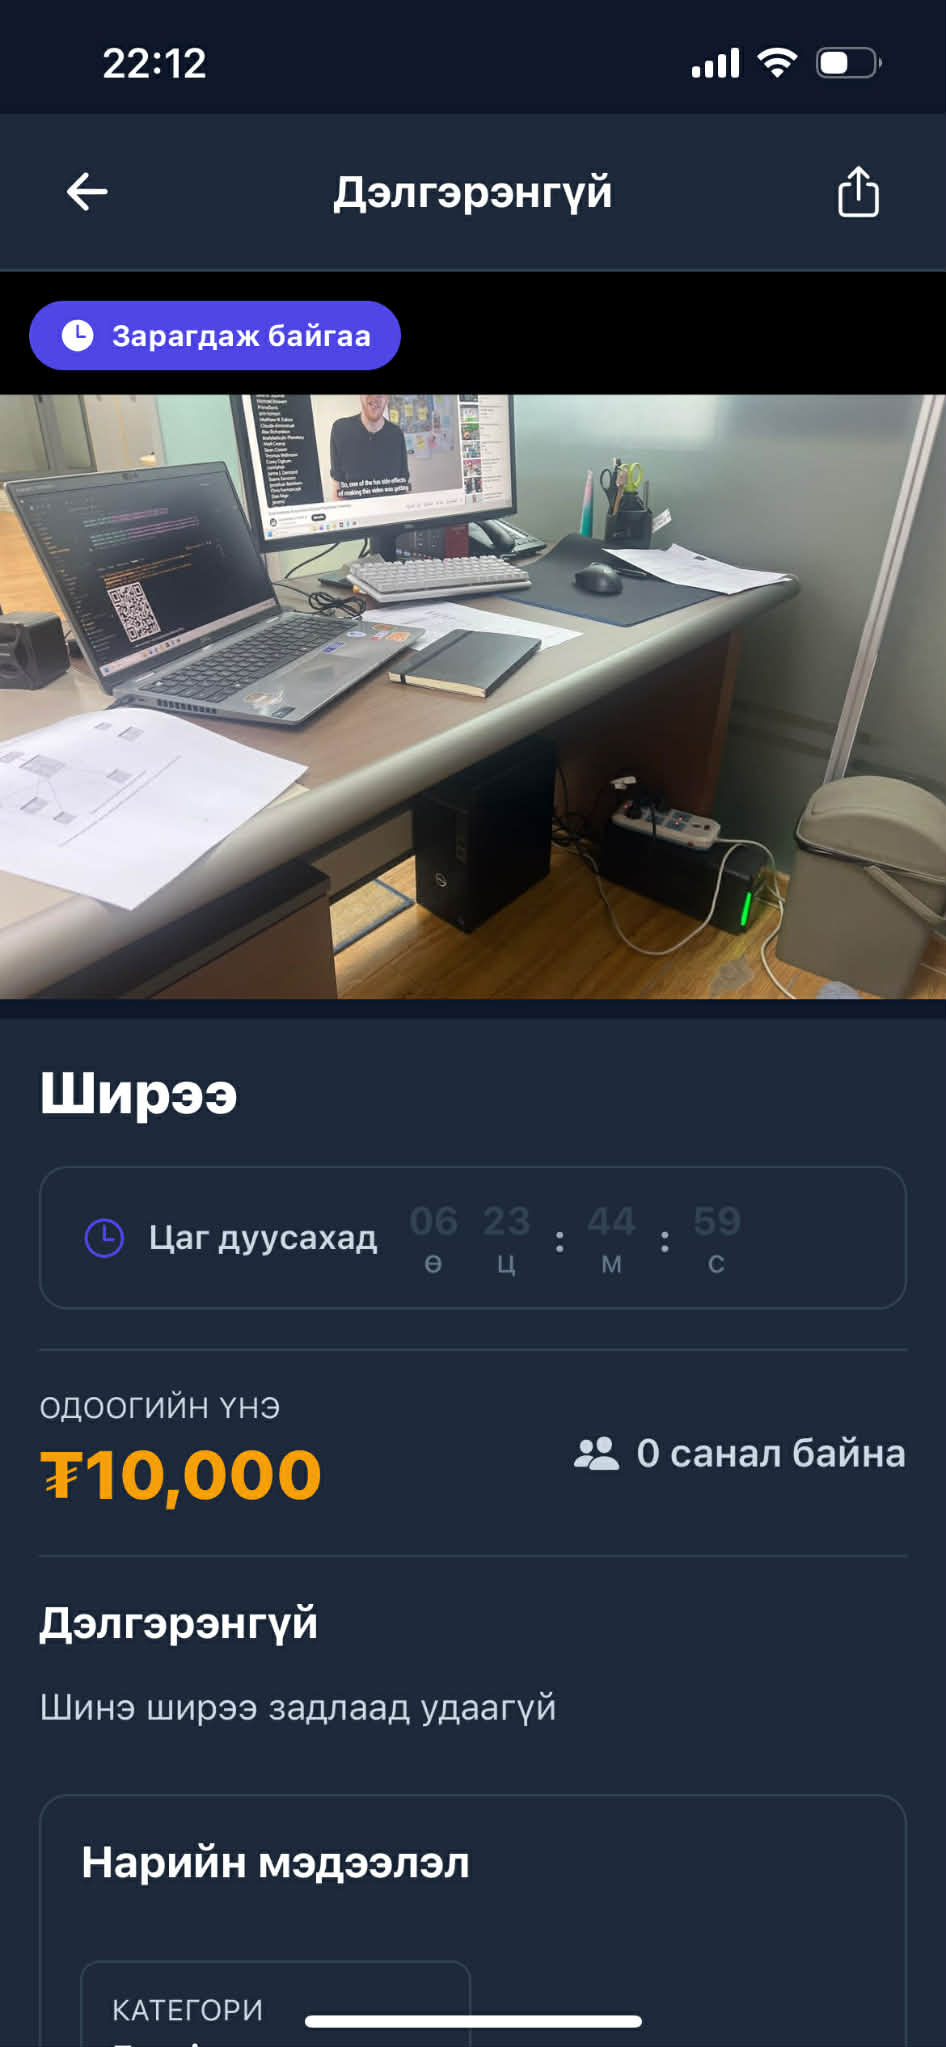
\includegraphics[width=\textwidth]{mobile_product.jpg}
    \caption{Бараан дэлгэрэнгүй — countdown таймер, дуудлагын мэдээлэл}
    \label{fig:mobile-product}
  \end{minipage}
\end{figure}

% ── Authentication flow ───────────────────────────────────────────────
\begin{figure}[H]
  \centering
  \begin{minipage}{0.45\textwidth}
    \centering
    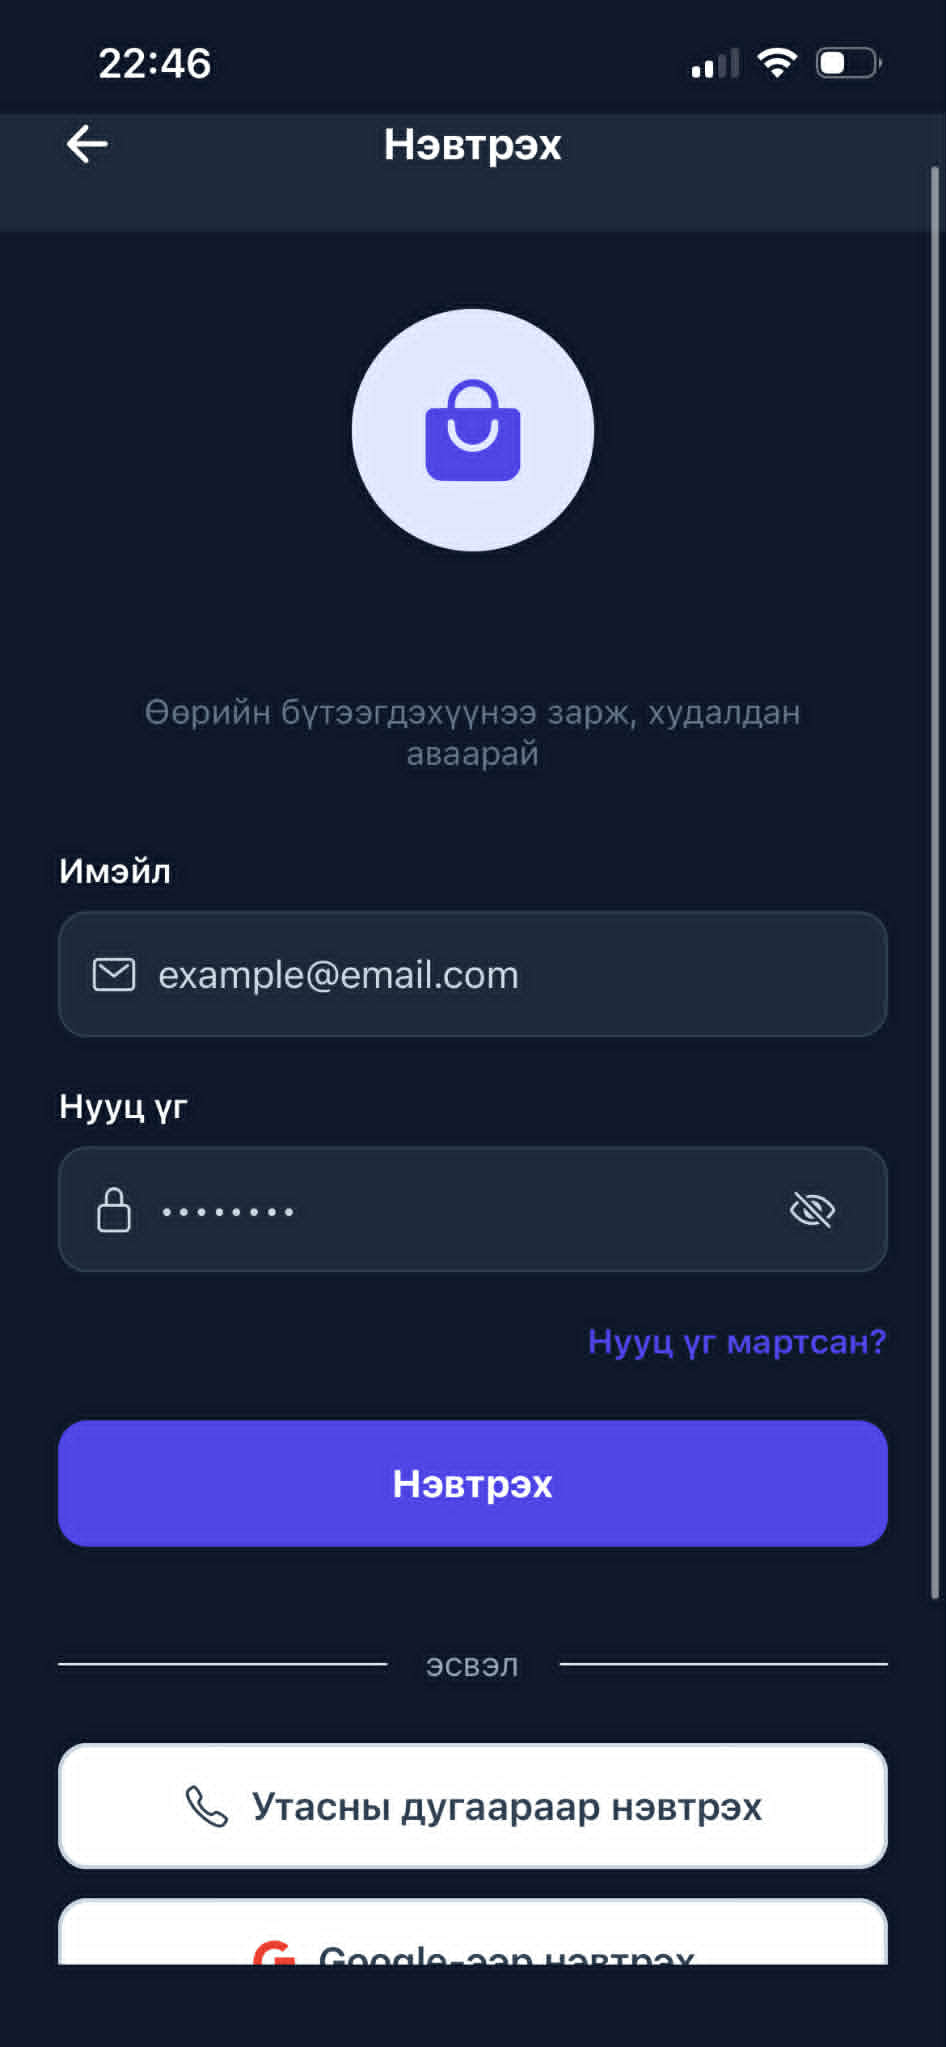
\includegraphics[width=\textwidth]{mobile_login.jpg}
    \caption{Нэвтрэх — имэйл, утас, Google OAuth}
    \label{fig:mobile-login}
  \end{minipage}
  \hfill
  \begin{minipage}{0.45\textwidth}
    \centering
    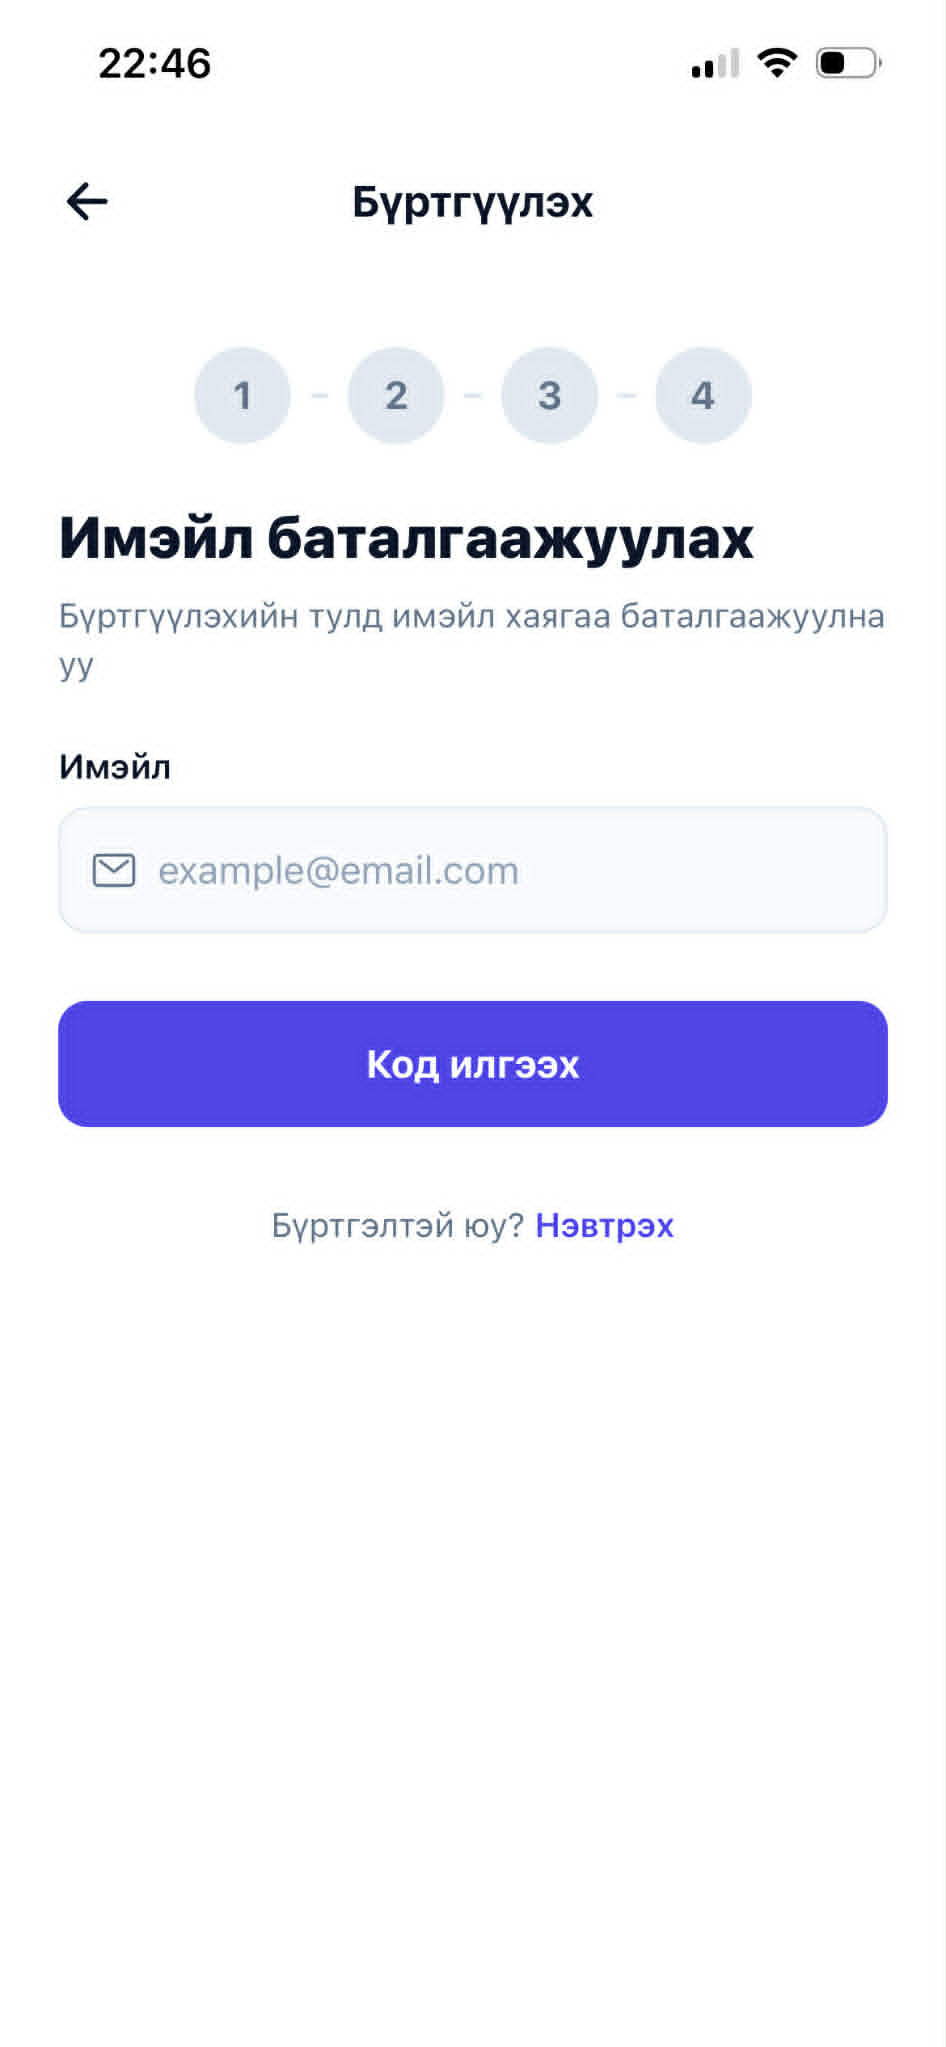
\includegraphics[width=\textwidth]{mobile_email.jpg}
    \caption{Бүртгэл — имэйл баталгаажуулах (1-р алхам)}
    \label{fig:mobile-email}
  \end{minipage}
\end{figure}

\begin{figure}[H]
  \centering
  \begin{minipage}{0.45\textwidth}
    \centering
    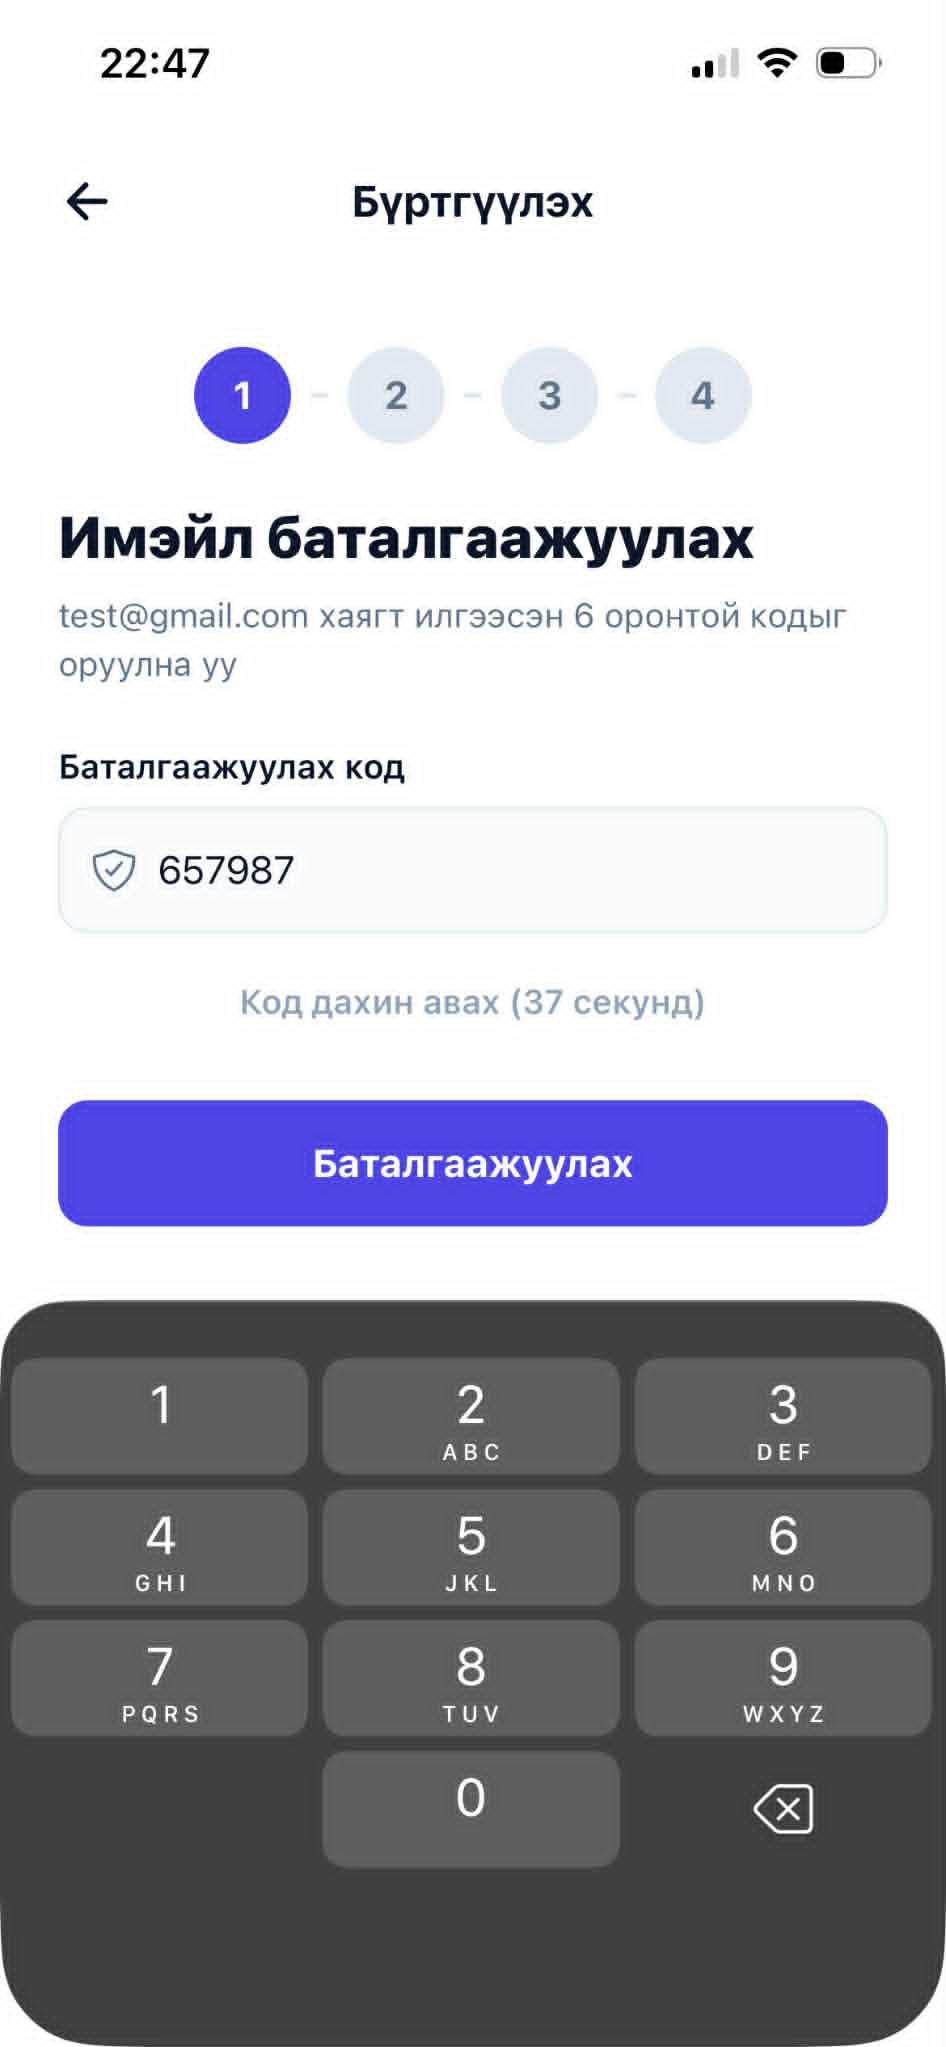
\includegraphics[width=\textwidth]{mobile_verification.jpg}
    \caption{Бүртгэл — баталгаажуулах код (2-р алхам)}
    \label{fig:mobile-verification}
  \end{minipage}
  \hfill
  \begin{minipage}{0.45\textwidth}
    \centering
    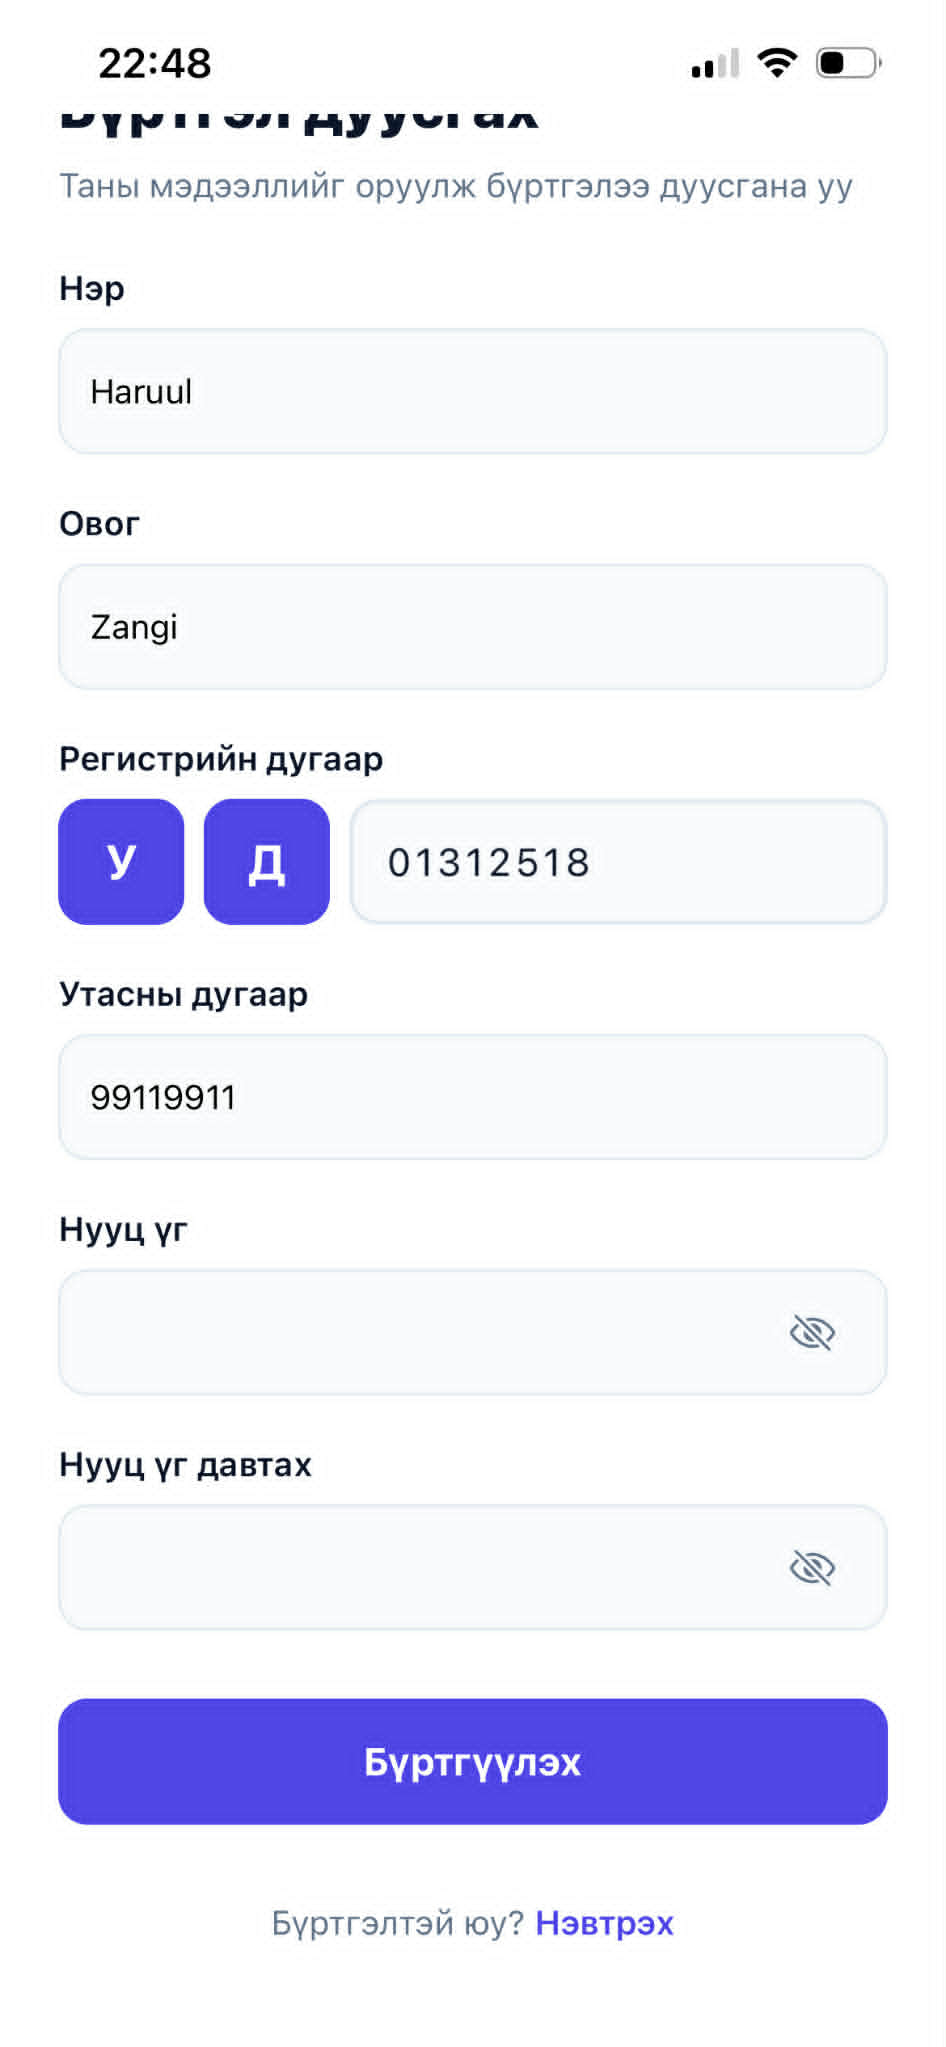
\includegraphics[width=\textwidth]{mobile_registration.jpg}
    \caption{Бүртгэл — регистрийн дугаар сонгогч (4-р алхам)}
    \label{fig:mobile-registration}
  \end{minipage}
\end{figure}

\begin{figure}[H]
  \centering
  \begin{minipage}{0.45\textwidth}
    \centering
    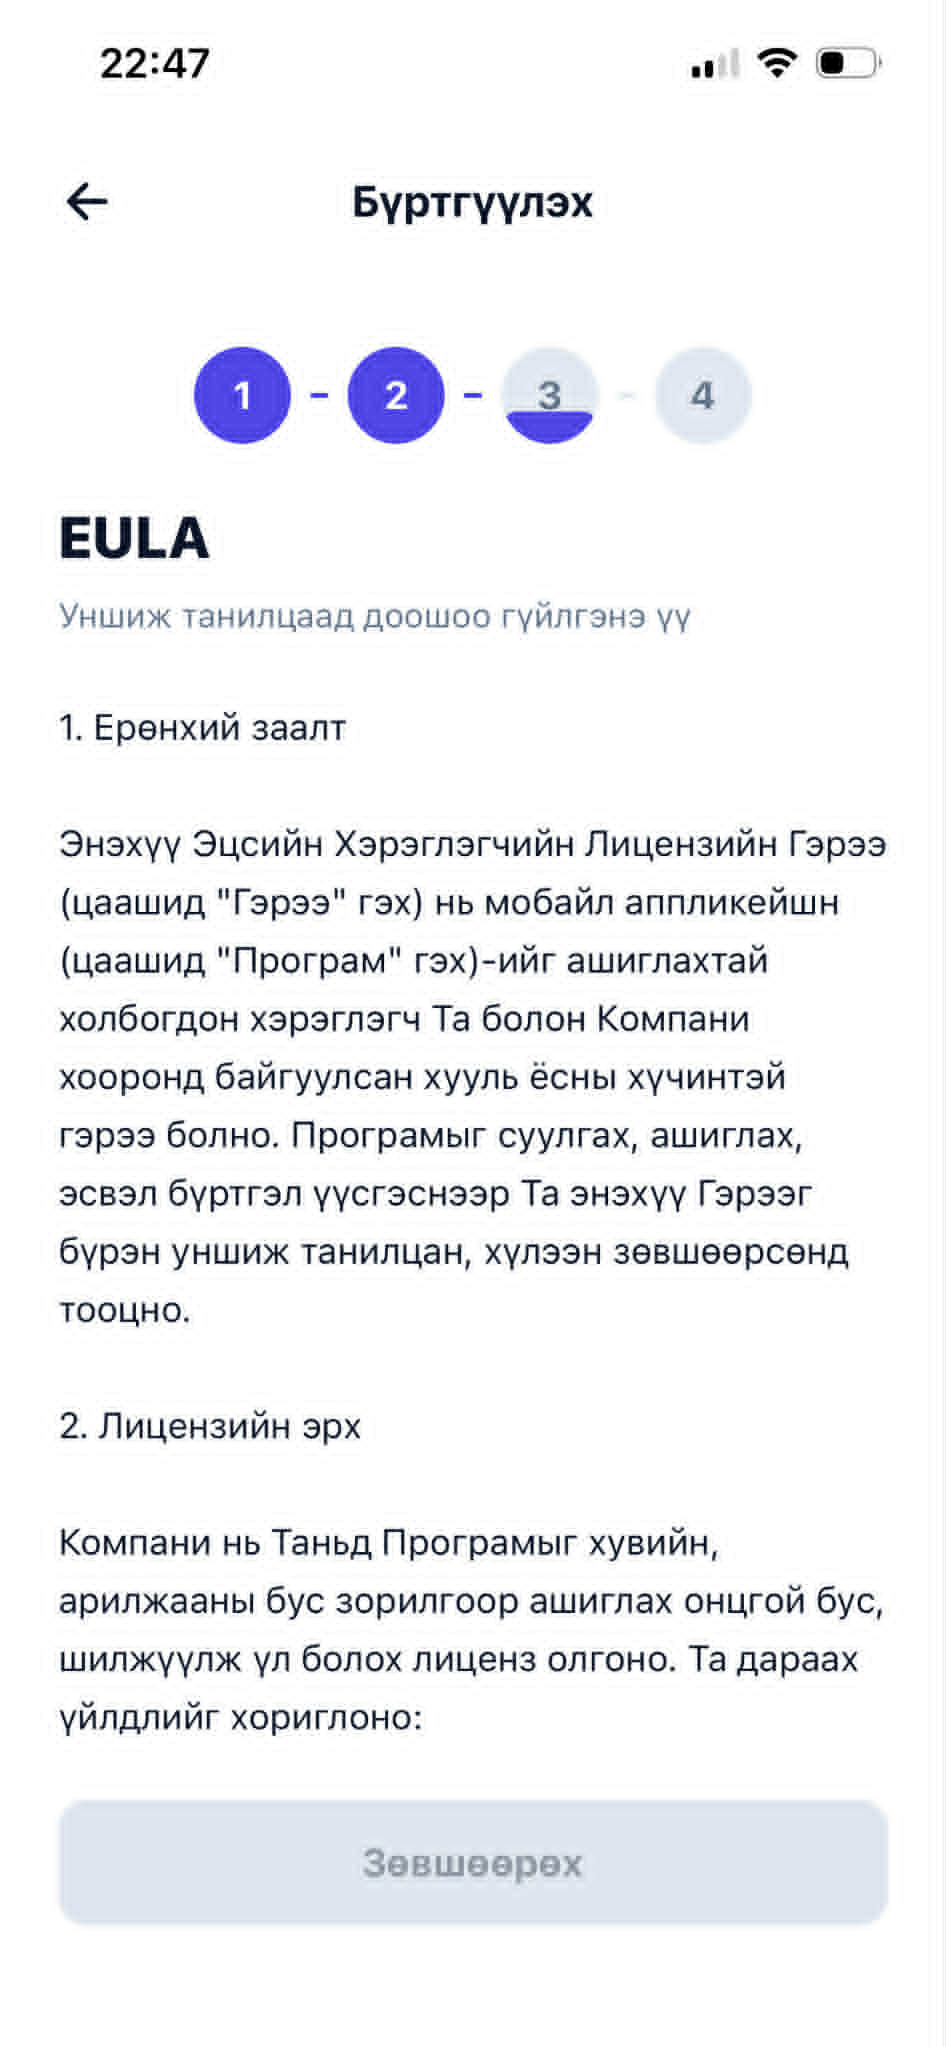
\includegraphics[width=\textwidth]{mobile_eula.jpg}
    \caption{Үйлчилгээний нөхцөл зөвшөөрөх (3-р алхам)}
    \label{fig:mobile-eula}
  \end{minipage}
  \hfill
  \begin{minipage}{0.45\textwidth}
    \centering
    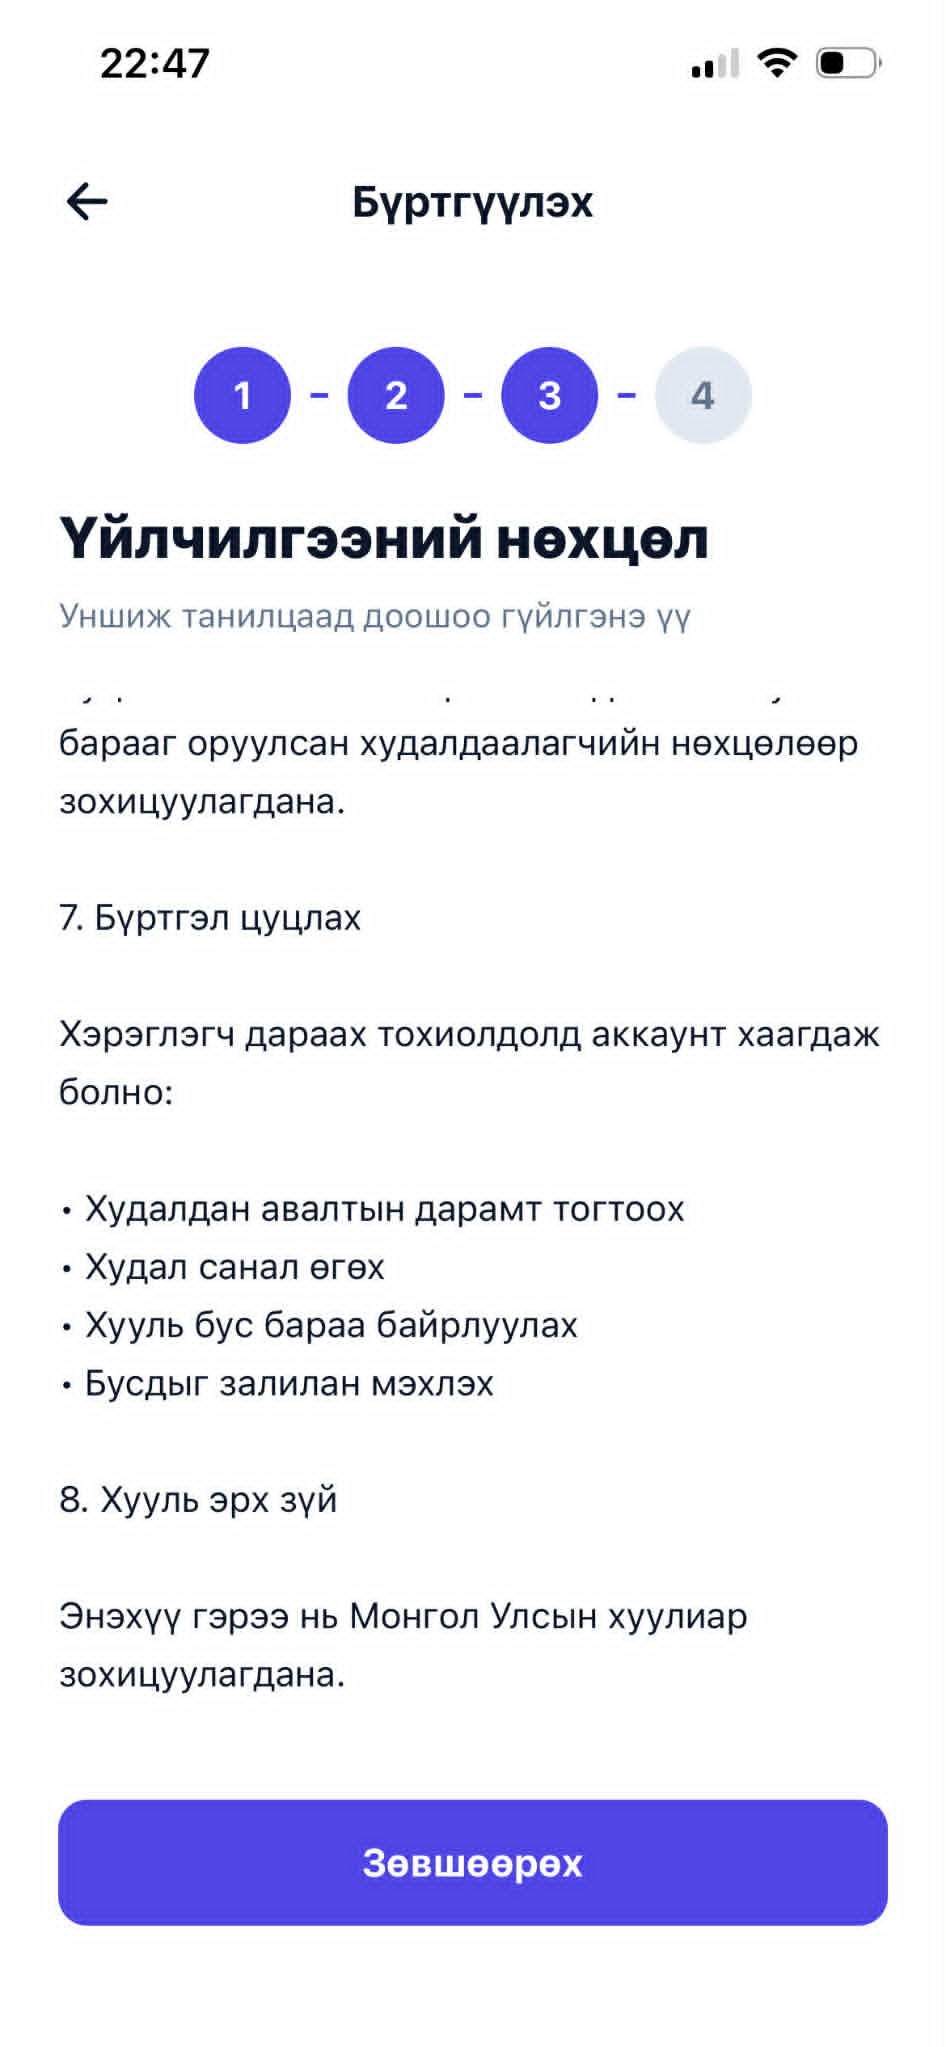
\includegraphics[width=\textwidth]{mobile_agreement.jpg}
    \caption{Гэрээний нөхцөл}
    \label{fig:mobile-agreement}
  \end{minipage}
\end{figure}

% ── Add product ───────────────────────────────────────────────────────
\begin{figure}[H]
  \centering
  \begin{minipage}{0.45\textwidth}
    \centering
    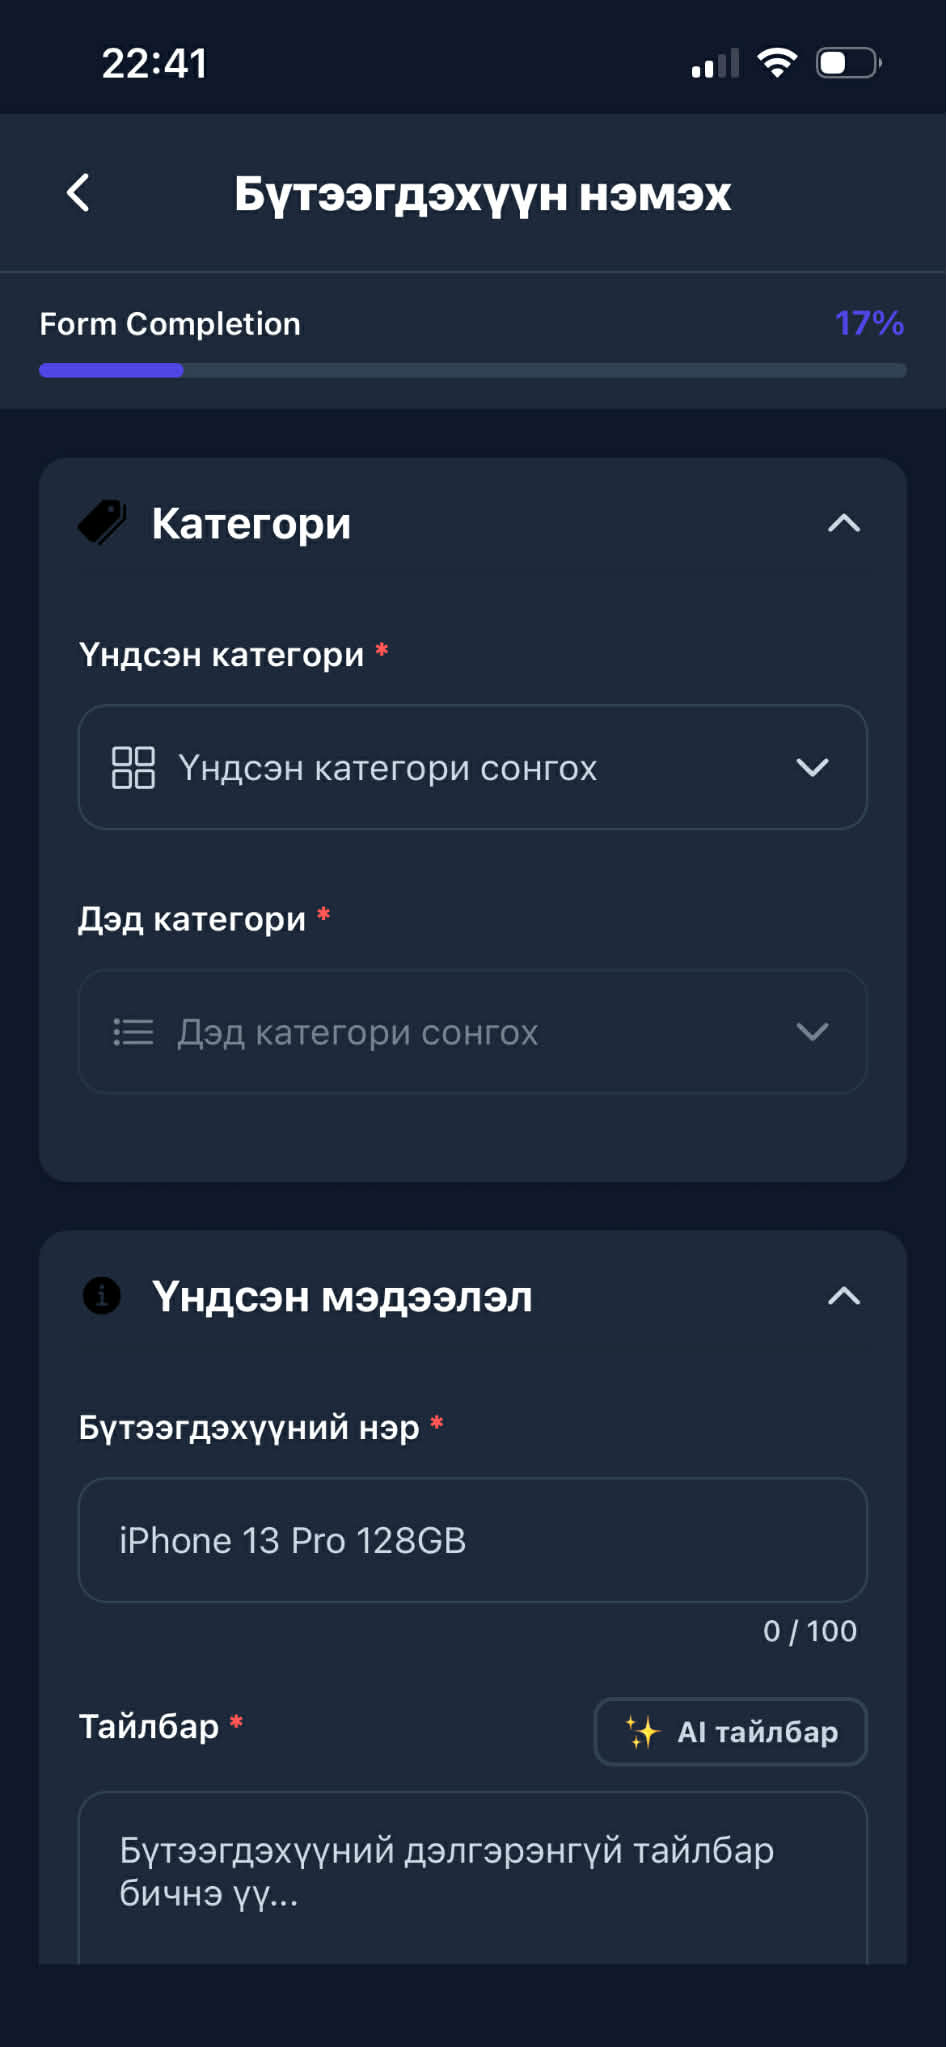
\includegraphics[width=\textwidth]{mobile_add_product1.jpg}
    \caption{Бараа нэмэх — категори, үндсэн мэдээлэл}
    \label{fig:mobile-add1}
  \end{minipage}
  \hfill
  \begin{minipage}{0.45\textwidth}
    \centering
    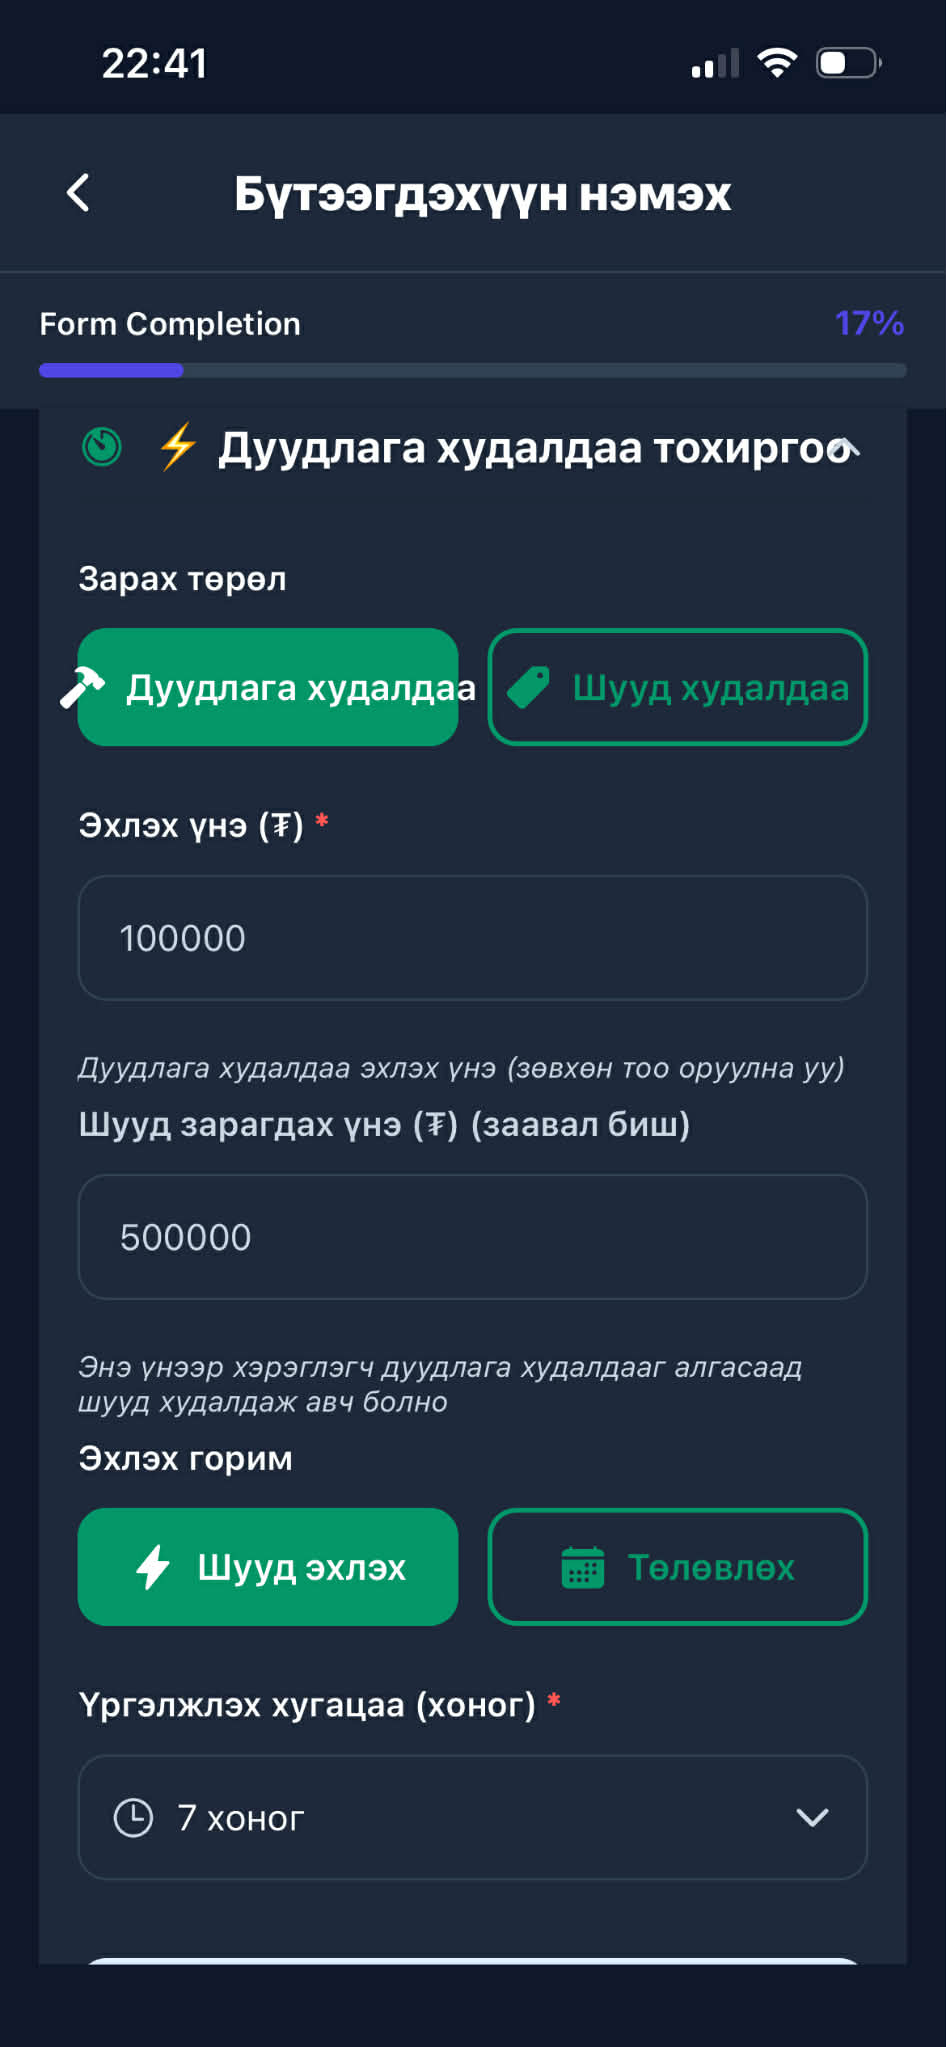
\includegraphics[width=\textwidth]{mobile_add_product2.jpg}
    \caption{Бараа нэмэх — үнэ, хугацааны тохиргоо}
    \label{fig:mobile-add2}
  \end{minipage}
\end{figure}

\subsection{Performance Optimization}

\begin{itemize}
  \item \texttt{FlatList} (бус \texttt{ScrollView}) — virtualization-аар RAM хэмнэх.
  \item \texttt{expo-image} — cache + placeholder.
  \item React.memo, useMemo, useCallback — re-render багасгах.
  \item Network retry + exponential backoff axios-interceptor дотор.
\end{itemize}

\section{Аюулгүй байдал ба нэвтрэлт}

\subsection{Хэрэглэгдэх технологи}

\begin{itemize}
  \item \textbf{JWT токен} — 7 өдрийн хугацаатай, stateless authentication.
  \item \textbf{bcrypt} — 10 round salt, нэг чиглэлийн хэш.
  \item \textbf{helmet} — HTTP security headers (XSS, clickjacking).
  \item \textbf{express-rate-limit} — IP бүрд минутанд 100 хүсэлт.
  \item \textbf{cors} — Cross-origin policy.
  \item \textbf{Mongoose strict mode} — NoSQL injection урьдчилан сэргийлэх.
\end{itemize}

\subsection{Алдааны тохиолдолд}

\begin{itemize}
  \item Токен байхгүй → \texttt{401 Unauthorized}
  \item Админ эрхгүй → \texttt{403 Forbidden}
  \item Буруу / истэк токен → \texttt{401} + \texttt{code: 'TOKEN\_EXPIRED'}
\end{itemize}

\section{Гадны интеграцууд}

\subsection{Google OAuth 2.0}

Frontend дээр Google Identity Services button → id\_token авах → server \texttt{google-auth-library}-аар verify → \texttt{googleId}-аар User хайх, олдохгүй бол auto-register → JWT буцаах.

\subsection{Cloudinary}

Multer + multer-storage-cloudinary ашиглан upload route дээр шууд Cloudinary руу stream. Transformation: \texttt{\{width: 1200, height: 1200, crop: 'limit', quality: 'auto'\}}.

\subsection{QPay}

\begin{enumerate}
  \item \texttt{POST /v2/auth/token} — Basic auth (username:password) → \texttt{access\_token} авах.
  \item \texttt{POST /v2/invoice} — Invoice үүсгэх → \texttt{qr\_image} (base64), \texttt{qr\_text}, bank deep links авах.
  \item Хэрэглэгч банкны аппликейшнаар QR уншиж төлбөр.
  \item \texttt{GET /v2/payment/check} — 3 секунд тутам polling, count > 0 бол paid.
  \item Webhook \texttt{POST /api/webhook/qpay-webhook} — QPay callback, balance шинэчлэх.
\end{enumerate}

\section{Deployment ба DevOps}

\begin{itemize}
  \item \textbf{Backend}: Render.com — Auto-deploy from GitHub \texttt{main} branch.
  \item \textbf{Database}: MongoDB Atlas M0 (free).
  \item \textbf{Frontend}: Vercel — \texttt{vite build}, static hosting + CDN.
  \item \textbf{Mobile}: Expo EAS Build — iOS .ipa, Android .apk/.aab.
  \item \textbf{Logs}: Winston + log rotation.
\end{itemize}

\section{Бүлгийн дүгнэлт}

Энэ бүлэгт системийн гурван үндсэн бүрэлдэхүүний хөгжүүлэлтийн нарийвчилсан тайлбарыг өгсөн. Технологийн сонголтын үндэслэл, модулиудын дотоод бүтэц, bid placement логикийн псевдо код, REST API endpoint-ын зохион байгуулалт, Socket.IO event-үүд, аюулгүй байдлын механизм, QPay болон Cloudinary интеграц зэргийг бүгдийг тусгасан.

% =====================================================================
%  CHAPTER 4 — TESTING
% =====================================================================
\chapter{Туршилт, үр дүн}

Туршилт нь 4 үндсэн хэсэгт хуваагдана: (1) Backend API тест, (2) Unit тест, (3) Integration тест, (4) Мобайл тест.

\section{Системийн ажиллагааны тест}

\subsection{API Endpoint тест (Insomnia)}

\begin{table}[H]
  \centering
  \caption{Хэрэглэгчийн API туршилтын үр дүн}
  \label{tab:user-api-test}
  \begin{tabularx}{\textwidth}{C{0.5cm}C{1.2cm}L{5cm}C{2cm}C{1.5cm}L{3.5cm}}
    \toprule
    \textbf{\#} & \textbf{Арга} & \textbf{Endpoint} & \textbf{Хүлээгдэж буй} & \textbf{Үр дүн} & \textbf{Тайлбар} \\
    \midrule
    1 & POST & /api/users/register & 201 & 201 & Бүртгэл амжилттай \\
    2 & POST & /api/users/login & 200+token & 200+token & JWT буцсан \\
    3 & GET & /api/users/getuser & 200 & 200 & Токентой хүсэлт \\
    4 & GET & /api/users/getuser & 401 & 401 & Токенгүй татгалзасан \\
    5 & GET & /api/users/userbalance & 200 & 200 & Баланс буцсан \\
    6 & POST & /api/users/send-code & 200 & 200 & Код илгээгдсэн \\
    7 & POST & /api/users/verify-email & 200 & 200 & И-мэйл баталгаажсан \\
    8 & POST & /api/users/forgot-password & 200 & 200 & Reset и-мэйл явсан \\
    9 & PUT & /api/users/photo & 200 & 200 & Зураг шинэчлэгдсэн \\
    10 & GET & /api/users/allusers & 200 & 200 & Зөвхөн админ \\
    \bottomrule
  \end{tabularx}
\end{table}

\begin{table}[H]
  \centering
  \caption{Барааны API туршилтын үр дүн}
  \label{tab:product-api-test}
  \begin{tabularx}{\textwidth}{C{0.5cm}C{1.2cm}L{5cm}C{2cm}C{1.5cm}L{3.5cm}}
    \toprule
    \textbf{\#} & \textbf{Арга} & \textbf{Endpoint} & \textbf{Хүлээгдэж буй} & \textbf{Үр дүн} & \textbf{Тайлбар} \\
    \midrule
    1 & GET & /api/product/products & 200 & 200 & Бүх бараа буцсан \\
    2 & POST & /api/product & 201 & 201 & Бараа нэмэгдсэн \\
    3 & POST & /api/product & 401 & 401 & Токенгүй татгалзасан \\
    4 & GET & /api/product/my & 200 & 200 & Өөрийн бараа \\
    5 & GET & /api/product/:id & 200 & 200 & Дэлгэрэнгүй мэдээлэл \\
    6 & GET & /api/product/:id & 404 & 404 & Буруу ID \\
    7 & PUT & /api/product/:id & 200 & 200 & Мэдээлэл шинэчлэгдсэн \\
    8 & DELETE & /api/product/:id & 200 & 200 & Бараа устгагдсан \\
    9 & POST & /api/product/suggest-category & 200 & 200 & AI ангилал санал \\
    \bottomrule
  \end{tabularx}
\end{table}

\begin{table}[H]
  \centering
  \caption{Дуудлага худалдааны API туршилтын үр дүн}
  \label{tab:bid-api-test}
  \begin{tabularx}{\textwidth}{C{0.5cm}C{1.2cm}L{5cm}C{2cm}C{1.5cm}L{3.5cm}}
    \toprule
    \textbf{\#} & \textbf{Арга} & \textbf{Endpoint} & \textbf{Хүлээгдэж буй} & \textbf{Үр дүн} & \textbf{Тайлбар} \\
    \midrule
    1 & POST & /api/bidding & 200 & 200 & Үнэ санал амжилттай \\
    2 & POST & /api/bidding & 400 & 400 & Хангалтгүй баланс \\
    3 & GET & /api/bidding/:productId & 200 & 200 & Үнийн түүх буцсан \\
    4 & GET & /api/bidding/my & 200 & 200 & Өөрийн санал \\
    5 & GET & /api/bidding/my-wins & 200 & 200 & Ялсан дуудлага \\
    6 & GET & /api/bidding/my-losses & 200 & 200 & Ялагдсан дуудлага \\
    \bottomrule
  \end{tabularx}
\end{table}

Нийт \textbf{34 API endpoint}-ийг Insomnia-аар шалгасан бөгөөд бүгд хүлээгдэж буй хариуг буцаасан.

\subsection{Unit тест (Jest)}

\subsubsection{BiddingController тест}

\begin{itemize}
  \item \textbf{TC-1}: Хүчинтэй санал → 201 + Bidding баримт
  \item \textbf{TC-2}: Хангалтгүй balance → 400 'Insufficient balance'
  \item \textbf{TC-3}: Хэт бага үнэ → 400 'Bid too low'
  \item \textbf{TC-4}: Дуусчихсан auction → 400 'Auction not active'
  \item \textbf{TC-5}: Хугацаа хэтэрсэн → 400 'Auction expired'
  \item \textbf{TC-6}: Өөрийн бараа дээр санал → 403 'Cannot bid on own product'
\end{itemize}

Бүгд expected үр дүнг өгсөн. Coverage: backend нь \textbf{65\% line coverage}, controller layer \textbf{80\%+}.

\subsection{Integration тест}

Supertest + in-memory MongoDB (\texttt{mongodb-memory-server}) ашиглан real HTTP request → real DB → real response. Нийт \textbf{18 интеграц тест} бүх эерэг үр дүн өгсөн.

\subsection{Мобайл аппликейшны тест}

\begin{itemize}
  \item iPhone (iOS 14+) — iPhone 12, iPhone 14 Pro
  \item Android (Android 11+) — Samsung Galaxy A52, Xiaomi Redmi Note 11
  \item Tablet — iPad Air, Samsung Tab S6
  \item Өөр өөр дэлгэцийн хэмжээ (320px--1024px)
\end{itemize}

\section{Гүйцэтгэлийн (Performance) тест}

\begin{table}[H]
  \centering
  \caption{Endpoint бүрийн гүйцэтгэлийн дундаж үзүүлэлт}
  \label{tab:performance}
  \begin{tabularx}{\textwidth}{L{5cm}C{2cm}C{2.5cm}C{2.5cm}C{2cm}}
    \toprule
    \textbf{Endpoint} & \textbf{RPS} & \textbf{Avg latency} & \textbf{P95 latency} & \textbf{Алдаа \%} \\
    \midrule
    GET /api/product (list 20) & 250 & 85 мс & 220 мс & 0\% \\
    GET /api/product/:id & 380 & 60 мс & 150 мс & 0\% \\
    POST /api/users/login & 120 & 180 мс & 380 мс & 0\% \\
    POST /api/bidding & 200 & 110 мс & 290 мс & 0\% \\
    GET /api/notifications & 300 & 75 мс & 180 мс & 0\% \\
    \bottomrule
  \end{tabularx}
\end{table}

P95 < 400 мс — зорилт болгож тогтоосон 500 мс-ийн хязгааравас доогуур байна.

Real-time bid latency: Socket.IO дээр дунджаар \textbf{45--80 мс} (local network); хэрэглэгчид өөрчлөлтийг \textbf{< 1 секунд} дотор хүлээж авна.

\section{Аюулгүй байдлын тест (OWASP Top-10)}

\begin{table}[H]
  \centering
  \caption{OWASP Top-10 хамгаалалтын тойм}
  \label{tab:owasp}
  \begin{tabularx}{\textwidth}{L{3.5cm}L{4cm}L{6cm}}
    \toprule
    \textbf{OWASP эрсдэл} & \textbf{Тайлбар} & \textbf{Хэрэгжүүлсэн хамгаалалт} \\
    \midrule
    A01: Broken Access Control & Зөвшөөрөл алдагдах & Role-based middleware, ownership check \\
    A02: Cryptographic Failures & Сул хэшлэлт & bcrypt 10 round, HTTPS only \\
    A03: Injection & NoSQL injection & Mongoose strict mode, sanitize input \\
    A05: Security Misconfiguration & Default config & helmet, .env, no debug in prod \\
    A06: Vulnerable Components & Хуучин npm & \texttt{npm audit}, Dependabot \\
    A07: Auth Failures & Brute force & express-rate-limit, account lockout \\
    A09: Logging Failures & Аудит дутагдал & Winston logs, Sentry \\
    \bottomrule
  \end{tabularx}
\end{table}

\section{Зорилтын биелэлт}

\begin{table}[H]
  \centering
  \caption{Зорилтын биелэлт}
  \label{tab:objectives}
  \begin{tabularx}{\textwidth}{C{0.5cm}L{4.5cm}C{1.5cm}L{6cm}}
    \toprule
    \textbf{\#} & \textbf{Зорилт} & \textbf{Биелэлт} & \textbf{Тайлбар} \\
    \midrule
    1 & Real-time data & \ding{51} & Socket.IO bidUpdate, < 1 сек \\
    2 & QPay интеграц & \ding{51}* & Архитектур бэлэн, sandbox тест хийгдсэн \\
    3 & Google OAuth & \ding{51} & Веб, мобайл дээр хэрэгжсэн \\
    4 & Автомат дуудлага & \ding{51} & Cron job, ялагч тогтоох, balance шилжүүлэх \\
    5 & MongoDB & \ding{51} & Atlas cluster, 11 collection \\
    6 & Аюулгүй байдал & \ding{51} & JWT+bcrypt+helmet, P95 < 400 мс \\
    7 & Тест & \ding{51} & Unit + Integration + API + Mobile \\
    \bottomrule
    \multicolumn{4}{l}{\footnotesize * QPay sandbox орчинд тестлэгдсэн; merchant agreement-г дуусгах шаардлагатай.}
  \end{tabularx}
\end{table}

\section{Хязгаарлалт ба мэдэгдсэн дутагдал}

\begin{itemize}
  \item \textbf{QPay} — Sandbox орчинд тестлэгдсэн; merchant agreement байгуулагдаагүй.
  \item \textbf{Live video streaming} — Shopee-маягийн video auction нь ирээдүйн ажилд орсон.
  \item \textbf{i18n} — Англи хэлний UI \textasciitilde80\% хүрсэн.
  \item \textbf{Penetration test} — Мэргэжлийн гуравдагч тал хийгдээгүй.
  \item \textbf{Offline mode} — Хязгаарлагдмал; placeBid offline-д ажиллахгүй.
\end{itemize}

\section{Бүлгийн дүгнэлт}

Системийг API, юнит, интеграц, мобайл, гүйцэтгэл, аюулгүй байдлын зургаан өнцгөөс шалгасан. Бүх тогтоосон зорилт биелэгдсэн бөгөөд гүйцэтгэлийн зорилго (P95 < 500 мс, real-time < 1 сек) хэвээр давамгайлж байна.

% =====================================================================
%  CONCLUSION
% =====================================================================
\chapter*{Дүгнэлт}
\addcontentsline{toc}{chapter}{Дүгнэлт}
\markboth{ДҮГНЭЛТ}{}

Энэхүү төслийн хүрээнд онлайн дуудлага худалдааны цогц систем амжилттай хөгжүүлсэн. Систем нь веб апликейшн, мобайл апликейшн, backend сервер гэсэн 3 үндсэн хэсгээс бүрдэж, хэрэглэгчдэд бүрэн функциональ, найдвартай, хүртээмжтэй үйлчилгээ үзүүлж байна.

\section*{Тоон үр дүн}

\begin{table}[H]
  \centering
  \caption{Системийн нэгтгэсэн тоон үр дүн}
  \label{tab:summary}
  \begin{tabularx}{\textwidth}{L{6cm}L{6cm}}
    \toprule
    \textbf{Хэмжүүр} & \textbf{Утга} \\
    \midrule
    Платформ & 3 (Web, iOS, Android) \\
    MongoDB collection & 11 \\
    REST endpoint & 34+ \\
    Socket.IO event & 7 \\
    Категори & 66 \\
    API P95 latency & $< 400$ мс \\
    Real-time bid latency & $< 1$ секунд \\
    Тестийн coverage (backend) & 65\% \\
    Кодын мөр (нийт) & \textasciitilde12,000 \\
    \bottomrule
  \end{tabularx}
\end{table}

\section*{Давуу талууд}

\begin{itemize}
  \item \textbf{Multi-platform} — Веб, iOS, Android гурван платформ дээр ажилладаг.
  \item \textbf{Real-time систем} — Socket.IO ашиглан үнийн өөрчлөлтийг цаг алдалгүй хүргэдэг.
  \item \textbf{Монгол зах зээлд тохирсон} — 66 категори, төгрөг валют, Монгол хэл дэмжлэг.
  \item \textbf{AI технологи} — Категори автоматаар санал болгох систем.
  \item \textbf{Trust score систем} — Хэрэглэгчийн найдвартай байдлыг тоон утгаар хэмжих механизм.
\end{itemize}

\section*{Ирээдүйд хийж болох хөгжүүлэлтүүд}

\begin{itemize}
  \item \textbf{Live video streaming} — WebRTC эсвэл Twilio Live Video ашиглан.
  \item \textbf{QPay бодит орчин} — Merchant agreement, production deployment.
  \item \textbf{AI чат бот} — OpenAI/Claude-д суурилсан хэрэглэгчийн тусламжийн bot.
  \item \textbf{Анти-снайпинг} — Сүүлийн 60 секундэд санал орвол хугацаа +30 сек сунгах.
  \item \textbf{Блокчэйн} — Smart contract-аар автомат settlement, NFT auction.
  \item \textbf{Multi-currency} — USD, CNY зэрэг гадаад валют, бодит цагийн ханш.
  \item \textbf{Penetration testing} — Мэргэжлийн ИБ багаас OWASP ASVS дагуу.
\end{itemize}

\section*{Төслийн ач холбогдол}

Дотоодын зах зээлд \textit{жинхэнэ live auction}-ыг бодит цагаар, гар утсаар хүртээмжтэй, Монгол хэл-төгрөгийн орчинд эрхлэн явуулах систем нь өмнө бараг байгаагүй. Энэ ажил нь дотоодын инженерийн нийгэмлэгт \textit{cross-platform + real-time + cloud-native} архитектурын бодит жишээ болж өгснийхөө хувьд онол-практикийн талаас аль алинд хувь нэмэр оруулсан гэж үзэж байна.

Vickrey-Myerson-ы аукшины теорийн revenue equivalence зарчмыг English auction хэлбэрээр практикт буулгаж, Akerlof-ийн мэдээллийн тэгш бус байдлыг trust score системээр шийдвэрлэх оролдлого — эдийн засгийн онолын зарчмыг компьютерийн шинжлэх ухаантай хослуулан хэрэгжүүлсэн нэгэн жишээ болсон гэдэгт итгэлтэй байна.

% =====================================================================
%  BIBLIOGRAPHY
% =====================================================================
\chapter*{Ашигласан эх сурвалж}
\addcontentsline{toc}{chapter}{Ашигласан эх сурвалж}
\markboth{АШИГЛАСАН ЭХ СУРВАЛЖ}{}

\begin{enumerate}
  \item Vickrey, W. (1961). Counterspeculation, auctions, and competitive sealed tenders. \textit{The Journal of Finance}, 16(1), 8--37.
  \item Myerson, R. B. (1981). Optimal auction design. \textit{Mathematics of Operations Research}, 6(1), 58--73.
  \item Akerlof, G. A. (1970). The market for "lemons": Quality uncertainty and the market mechanism. \textit{The Quarterly Journal of Economics}, 84(3), 488--500.
  \item Mozilla Developer Network. (2024). \textit{WebSocket API}. Retrieved from https://developer.mozilla.org/en-US/docs/Web/API/WebSocket
  \item Node.js Foundation. (2024). \textit{Node.js Documentation v20 LTS}. Retrieved from https://nodejs.org/docs
  \item MongoDB, Inc. (2024). \textit{MongoDB Manual 7.0}. Retrieved from https://www.mongodb.com/docs
  \item Expo. (2024). \textit{Expo Documentation --- SDK 54}. Retrieved from https://docs.expo.dev
  \item React Native. (2024). \textit{React Native Docs 0.74}. Retrieved from https://reactnative.dev/docs
  \item Socket.IO. (2024). \textit{Socket.IO Documentation v4}. Retrieved from https://socket.io/docs/v4
  \item QPay Mongolia. (2024). \textit{QPay Merchant API Documentation}. Улаанбаатар: QPay ХХК.
  \item OWASP Foundation. (2021). \textit{OWASP Top Ten 2021}. Retrieved from https://owasp.org/Top10
  \item Cloudinary. (2024). \textit{Cloudinary Developer Documentation}. Retrieved from https://cloudinary.com/documentation
  \item Firebase. (2024). \textit{Firebase Documentation}. Retrieved from https://firebase.google.com/docs
  \item eBay Inc. (2023). \textit{eBay Annual Report 2023}. San Jose, CA.
  \item Mercari Inc. (2023). \textit{Mercari Group Annual Report 2023}. Tokyo, Japan.
  \item Shopee. (2024). \textit{Shopee Platform Overview}. Sea Limited, Singapore.
\end{enumerate}

\end{document}
